\documentclass{article}

\usepackage[utf8]{inputenc}
\usepackage{graphicx}
\usepackage{url}
\usepackage{color}
\usepackage{titlesec}
\usepackage{amsmath}
\usepackage{physics}
\usepackage{amsfonts}
\usepackage{hyperref}
\graphicspath{{../figures/}}

\title{notes: supersat}
\author{K. Latimer}
\date{Jan 13, 2020}

\begin{document}

\maketitle

\section{CAIPEEX}

\section{HALO}
\subsection{Data processing}
\begin{itemize}
	\item I did some manual cleanup on my Windows partition in earlier stages of the project for the HALO .ames files downloaded from the online database. The .ames conventions are defined \href{http://artefacts.ceda.ac.uk/formats/NASA-Ames/na-brief-guide.html}{here} and there was some degree of human error in following them. The correction process is documented in the ipython notebook file \texttt{HALO\_file\_processing.ipynb} and summarized in the text file ``HALO\_cleanup\_notes," both in notes/ subdirectory. The resulting raw data files are what I have saved in /data/halo/ames, and are the input for further processing by \texttt{halo\_data\_cleanup.py}. Note that some files from the GoAMAZON campaign have been excluded from that processing for various reasons (weird ames format, missing data, etc).
	\item 1/12/20: noticed some files had weird error values and changed them manually. Not sure why previous code didn't find those. Recorded in ``HALO\_cleanup\_notes".
	\item 1/14/20: noticed data missing in 3914. see ``HALO\_cleanup\_notes".
\end{itemize}

\subsection{Analysis}
For the record: feedback from R Weigel RE: disparate particle size PDFs between CAS and CDP instruments (bold emphasis mine):

{\itshape Related to the plots you have distributed (15 Nov 2019), it is not clear and difficult for us to judge whether the extracted particle concentrations were normalized to respective (and variable) bin width specified in the header of the data file.

The plots obviously show different size resolutions for the individual instruments, which disables a direct comparison of these data as the compared size bins are not equivalent.

One of our major concerns is that averaging over an entire flight causes an averaging over various cloud types and different developing stages of clouds. From take-off through landing, the averaging runs over liquid, mixed and ice phases at different atmospheric conditions and cloud ages. In addition to the non-equivalently binned data sets, the averaging over various cloud types could lead to misinterpretations. For instance, the spikes that you interpreted as CDP’s ``over-reporting" in sizes of 10, 20, 30 um (not size-resolved by the CAS) could result from (natural) cloud particle modes within different cloud types and/or at different development stages. \textbf{We suggest to limit the instrumental comparison to individual events of cloud encounters which may then be sorted by cloud types or atmospheric condition.}

Furthermore, \textbf{we suggest to consider differences in the data sets which may result from corrections of the sampled air volume based on the air speed. In terms of true air speed (TAS) or probe air speed (PAS), the data sets as given on the database are not equivalent. You can transfer the CAS data set to the standard of the CDP.} The needed calculations conclude from the instructions given in the data headers. However, for any comparison, the data sets should be consistent.

Finally, \textbf{we suggest once more to include also the NIXE-CAPS data sets} and to involve the colleagues in this discussion to better evaluate the deviation of the instruments’ data from each other also in the view of the instruments’ uncertainty.

From our point of view, at current stage, there is no unambiguous indication, which instrument is``over-" or ``under-reporting" something.}

\begin{itemize}
	\item 1/15/20: NIXE-CAPS data contains no time steps (for any flight) where all bins up to 52um diameter have non-error values (see \texttt{search\_NIXECAPS.py}). ADLR LWC values differ significantly from CAS and CDP...possibly includes rain droplets? See `comparelwc' figure. Also looked at effect of excluding size bins w/ mean diam $<$ 3um, and using `xi' correction factor on CAS; see `1001XX' figure.
	\item 1/17/20: reran \texttt{comparelwc\_set\_figsrc.py} --$>$ `v2' figure files. Just some aesthetic adjustments from v1: change colors, plot CAS second since it's usually smaller, sort time for 20140906 CAS data set. 
	\item 1/20/20: refigured raw data files to include lwc calculated values because it was taking too long to run those each time I made figures. General observations for comparelwc plots: 
		\begin{itemize}
			\item In general (see two notes down), ADLR lwc values from ames files are much larger than those calculated from CAS/CDP files...unclear what ADLR is including as liquid water but probably counts rain as well as cloud drops?
			\item Roughly three classifications: 1) missing data (either some or all of CAS and/or CDP) [0906, 0921, 0923, 0925, 1003, 1004]; 2) CAS and CDP data both present but peaks have significan mismatch [0919]; 3) CAS and CDP data both (reasonably) complete and peaks mostly match [0909, 0911, 0912, 0916, 0918, 0927, 0928, 0930, 1001]. 
			\item Out of the second two categories, the following have CAS/CDP peaks higher than ADLR lwc curve: 0912, 0916, 0918, 0928, 0930, 1001 - seems weird if ADLR is a superset of those as mentioned above
			\item Found some odd peak features with very small (generally under 1.e-5) lwc values when looking at 1001 dataset - code and figure (`v4comparelwc...') in scratch folder. 
		\end{itemize}
	\item 1/21/20: a few things...
		\begin{itemize}
			\item Following up on last point from yesterday: a couple of variations on comparelwc figure set: `v3': log scaling on y-axis...a bit hard to look at, hence `v4': zoom in to lower ($<$1.e-4) lwc regime. Noticed features that aren't visible at default scale, esp `several' (rough estimate only from skimming through) peaks still hitting 1.e-5 cutoff in: 0911, 0916, 0919, 0923, 0925, 0928, 1001. 
			\item I can't figure out a nice programatic way to separate cloud events without making a bunch of arbitrary decisions about selection parameters (peaks are not always cleanly delimited) so just doing manually for a couple of dates at this point. Chose 0909 and 1001 because CAS and CDP peaks roughly match so I can sort them out by eye; 1001 has the feature mentioned above that CAS/CDP lwcs can be higher than ADLR whereas 0909 does not, additionally 1001 has several of those small features discussed in preceeding point whereas 0909 has less - however, the total particle size PDFs we sent to Germany PI's are qualitatively similar so thought this was a good pair to examine side-by-side. 
		\end{itemize}
	\item 1/27/20: comparelwc set v5: include vertical wind velocity data on dual y-axis to figure out extent of error periods (hard to tell from looking at files)
	\item 1/28/20: Various notes on cloudevents figure set:
		\begin{itemize}
			\item Also added 0911 flight since a lot of vertical wind velocity data are missing from 1001 (no particular reason other than 0911 has roughly matching peaks between CAS and CDP and also roughly agrees with ADLR).
			\item Realized I should be plotting nconc/dr in upper left panel (just as I'm plotting nconc*r/dr in lower left panel)
			\item Can replace nconc/meanr vs t panel (lower right on top) with w/A vs t - generally A doesn't vary more than a few percent within a given cloud (order $10^{-2}$). Vertical wind velocity is missing for significant portion of all datasets...possibly concerning? Check with David (also see v5 comparelwc figure set).
			\item I went through all the cloudevent figures manually looking at nconc PDFs and particle size PDFs. I was looking for whether the curves for CAS and/or CDP were unimodal (i.e. a single global maximum, but allowed to be at the boundary of the domain). I excluded the lowest three bins for CAS and the lowest two bins for CDP (i.e., lower bin cutoff must be greater than 3um diameter (1.5um radius), per advice from Germany PIs). Results below in Table \ref{unimodal}. CAS definitely better by this metric; main problem with CDP seems to be 6th bin (11.8-15.6um radius range), which tends to report low relative to other bins. For cloud events where both instruments give unimodal curves, CAS pretty much always reports lower nconc and meanr (as we expect from LWC values).
		\end{itemize}
	\item 2/9/20: cloudevents set v2: corrected diameter to radius, corrected indexing bug for CAS in \texttt{get\_nconc\_vs\_t()}, calculated nconc and meanr with changed CAS correction factor and 3um bin cutoff (and graphed accordingly). Updated results similar; see Table \ref{unimodal2}\\
	\item 2/12/20: Several updates:
	\begin{itemize}
		\item Spent a good amount of time tweaking CAS vs CDP nconc and meanr scatter plots to make sure my results agreed with those previously found by Qindan in her Matlab code (\texttt{compare\_comparisons.py}). Note that her bin cutoffs for CAS were slighly different than the ones I had been using, which initially caused a discrepancy. But other than that it seems we match up fine.
		\item Realized I had forgotten to do a systematic study of the time offsets. Wrote some code to find the optimal offset for each flight date (\texttt{optimize\_offsets.py}), and incorporated those into the analysis. 
		\item Figure sets \texttt{meanr\_scatter} and \texttt{nconc\_scatter} show the effects of changing CAS correction factor, cutting off bins with particle diameters below 3um, and incorporating optimal time offsets described above (also all three of those things combined). Main takeaway: turns out we can acutally get pretty good aggreement in both quantities between the two instruments when all three correction schemes are put into place. Yay.
		\item There are a lot of figure versions right now. Descriptions: 
		\begin{itemize}
			\item \texttt{cloudevents\_set}: v3 - I can't find the documentation for this version in my notes but the figures look identical...; v4 - changed 20141001 offset to 2 per results from \texttt{optimize\_offsets}.
			\item The only one that really matters is v5 (output from most recent version of the code to date)
		\end{itemize}
	\end{itemize}
	\item 2/13/20:
	\begin{itemize}
		\item cloudevents set v5: no actual code changes, just to bring everything up to the same most-recent version number to date (TODO: create consistent git-integrated figure version system...)
		\item notes from meeting with David regarding scatter plots from yesterday:
		\begin{itemize}
			\item How to find the correct time offset for vertical wind velocity in supersaturation calculations???
			\item Make zoomed-in plots of LWC with vertical wind velocity to see where we're missing data (might need to do manual checks)
			\item Change nconc/meanr filters to an LWC filter (TODO)
		\end{itemize}
		\item removed old-version figure files from GitHub repo to meet file number limit
	\end{itemize}
	\item 2/17/20: Following David's comments from 2/13, changed filtering criteria for CAS/CDP scatter plots to look for LWC < 1.e-5 g/g. I did realize there is a complication here, which is that LWC is calculated using air density, derived from environmental data in ADLR files...so we still have the issue of not knowing the ``correct'' time alignment for the three instruments. Went ahead and made the plots anyway:
	\begin{itemize}
		\item meanr/nconc\_scatter set v6: filter on LWC, offset CAS time backwards
		\item meanr/nconc\_scatter set v7: filter on LWC, offset CDP time forwards
	\end{itemize}
	Those two versions are a bit sloppy in approach because they sync one out of CAS/CDP to ADLR for filtering, but the LWC values are calculated (in \texttt{halo\_data\_polish.py}) assuming all three synced together to begin with. My code for calculating LWC is slow so I need to either optimize it and rerun or just rerun when I have extra time (TODO). In any case, v6 and v7 described above give the same regression params to two decimal places, and look identical, so I don't think it's a priority (furthermore, it looks like $\rho_{air}$ doesn't change on timescales faster than a few minutes, whereas particle counts vary on the scale of seconds).

Slopes/correlations still look OK, but not quite as good. There's a strange blob of points in upper left quadrant of mean radius plots for a few flight dates; going to try to figure that out since it makes those regression params worse.

Also made meanr/nconc vs LWC plots out of curiosity but didn't see much. Also realized that the \texttt{optimize\_offsets} code was only filtering on meanr, so reran it with meanr \emph{and} nconc, as well as with LWC. Seems like the optimal offsets are pretty robust regardless.
	\item 2/18/20: trying to figure out blob. 
	\begin{itemize}
		\item meanr/nconc\_scatter set v8: LWC cutoff 3.e-5: gets rid of `blob' points (quantified using \texttt{figure\_out\_blob.py}: for all dates with visible blob combined, increasing cutoff from 1.e-5 to 3.e-5 removes 91\% of points in blob and only 16\% of points not in blob, where blob is defined as $r_{mean, CAS}$ between 6 and 10um, $r_{mean, CDP}$ between 12 and 17um).
		\item meanr/nconc\_scatter set v9: only nconc filter (no meanr): looks identical to v5 so only nconc matters.
	\end{itemize}
	\item 2/19/20: trying to understand relationship between nconc and LWC filtering:
	\begin{itemize}
		\item meanr/nconc\_scatter set v10: nconc cutoff 0.5 ptcls/ccm - analagous to v6/v7 wrt \% pts in blob
		\item meanr/nconc\_scatter set v11: nconc cutoff 1.5 ptcls/ccm - analogous to v8 wrt \% pts in blob
	\end{itemize}
	I am conceptually thinking of these two filters as roughly the same, therefore.

	Moving on to supersaturation (\texttt{ss\_scatter\_set\_figsrc.py}):
	\begin{itemize}
		\item v1: LWC cutoff 1.e-5, cas time offset back (cdp synced to adlr)
		\item v2: LWC cutoff 3.e-5, cas time offset back (cdp synced to adlr)
		\item v3: LWC cutoff 3.e-5, cdp time offset back (cas synced to adlr)
		\item v4: LWC cutoff 1.e-5, cdp time offset back (cas synced to adlr)
	\end{itemize}
	v2 and v3 show ``original data'' that looks more like what Qindan found before with the 10 ptcl/ccm cutoff (in agreement with above results), and are also more sensitive to the change in time offset schemes. David is confused/concerned about why v1 and v4 are \emph{not} sensitive to that...TODO: look at time scale of variations in vertical wind velocity / try making the plots with an extreme shift in adlr time offset and see what happens.
	\item 2/21/20: Follow up from above: looked at w data and time scale for variations is $\approx$ a few seconds so seems like ADLR offset should matter. Made the following versions of (\texttt{ss\_scatter\_set\_figsrc.py}):
	\begin{itemize}
		\item v5: ADLR at -10 second offset relative to CAS and CDP (CAS and CDP synced)
		\item v6: ADLR at -30 second offset relative to CAS and CDP (CAS and CDP synced)
	\end{itemize}
	We basically see no effect in the slope/correlation so David's concern is confirmed :/ 
	\item 2/27/20: notes from mtg with David: try doing correlation optimization wrt ADLR offset for LWC vs w, alternatively figure out a way to match downdrafts w/ cloud edges? unclear if that's really feasible though. (later thought 3/21/20: I feel like the correlations are not going to be that helpful since w deviates above and below 0 whereas LWC only deviates above...)
	\item 4/12/20: it's been a while but here we are. Sent Professors Jurkat and Weigel (et al on that email thread) a fairly extensive summary of results since January 2020 (all referenced figures in powerpoint in \texttt{pres} directory):\\

{\itshape Thank you for your patience as we have taken your thorough feedback into account in our analyses. In some cases, implementing the previous suggestions led to new questions for us, and we wanted to wait on sending this response until we felt we had a clearer picture of what was going on.

Here we are writing a summary of the points you all have raised throughout the correspondence, along with our subsequent findings. For brevity, we've included the figures in a single file, attached.

1. Various corrections to the datasets

In all cases here, we are filtering out points with liquid water content (LWC) less than 3*10$^-5$ g/g. Using a smaller LWC cutoff, we begin to see artifacts arising from the particle size distributions reported by the CDP instrument; see discussion in part (2)(A).

A. Commensurate sample volume correction factors

The ames files on the HALO database for the CAS instrument were corrected using the factor TAS/PAS, whereas for the CDP instrument they were corrected using the factor xi (as derived in Weigel et al (2016)). We re-corrected the CAS values using xi (provided as well in the datafiles), and generally don't see much improvement in correlation for number concentration (this correction doesn't change mean radius correlation since the volumetric factors cancel in the weighted average). See Figure 1.

B. Lower bound on particle size

As suggested by Dr. Jurkat, we performed the same comparison using only bins with a lower bound for droplet diameter greater than 3 um. This improves the value of the regression slope, but not the correlation, for number concentration (Figure 2), and nearly eliminates the constant offset between CAS and CDP mean radius (Figure 3).

C. Time offset between instruments

We also reran the analysis after offsetting the instrument times relative to one another such that the correlation between number concentration and mean radius measurements was optimized (these offsets varied across flight dates; see Figure 4). This correction yielded a significant improvement in agreement for number concentration (Figure 5), although not for mean radius (Figure 6).  Unfortunately, it's not clear to us how we should correctly sync CAS and CDP measurements to other instruments (in particular ADLR, which records most of the basic environmental variables).

The combined effect of corrections described in (A), (B), and (C) is shown in Figure 7. We also have analogues of Figures 1-6 for each individual flight date, and are happy to share those.

2. Cloud-by-cloud analysis

We were hoping to understand why the CDP instrument seems to report multi-modal cloud droplet size distributions, and Dr. Weigel suggested we analyze individual cloud events for each flight. We did so (working with the fully-corrected data described in part (1)), and an example plot is shown in Figure 8. We can provide the entire set upon request, but since there are many of them, we will summarize our main observations here:

A. We find CDP consistently reports bi- or multi-modal cloud droplet size distributions, even at the level of individual clouds (we are accounting for the variable bin size ranges when computing these distributions). For instance, on the 09 Sept flight, we found that about half of the CDP size distributions are non-unimodal, whereas all of the CAS size distributions are unimodal. This effect is most apparent in the mean cloud droplet size data at low LWC; if we use an LWC cutoff of 1*10$^-5$ (rather than 3*10$^-5$ as in part (1)), we see the cluster of points with anomalously high mean radius reported by CDP, as visible in Figure 9.

B. While LWC values reported by CAS and CDP are generally in good agreement (up to the ~1 second time offsets described in part (1)), there is one flight date (19 Sept) where they differ significantly even though neither reports error values, see Figure 10.

3. Comparison with other instruments

The only other bin-resolved cloud droplet data available in the online dataset from the GoAmazon field campaign was the NIXE-CAPS set. We did not find those files to be useful, due to high error rates. In particular, there were no timesteps in any of the flight dates where non-error-valued data were present for the whole particle size range of interest (3 um - 50 um diameter).

We did find (non-bin-resolved) LWC data in the ADLR set. However, it appears those measurements include rain droplets as well as cloud droplets, since the LWC values are considerably higher than those we calculated using the CAS and CDP sets (referring back to Figures 8 and 10).}\\

	\indent Selected points of feedback after this message:
	\begin{itemize}
		\item \emph{There are hotwire LWC measurements available. The hotwire was mounted on the CAS-DPOL but is an independent LWC measurement.  Ramon Braga also compared these in his paper with the CAS measurements (see plot below).} 
		\item \emph{We also have information on the phase and can thus apply a binning to either ice phase or liquid phase.  The current binning is chosen such that the ice and liquid can both be unambiguously detected. The consequence is a reduced size resolution in the lower size range. I can give you recommendations on how to do the binning. Once this is done, we can talk again about the comparison of the mean radius. As far as I remember there have been a few differences when going to higher MVDs.} 
		\item \emph{What might help is to compare the PAS (measured by the CAS) with the TAS of HALO and synchronize it with respect to level changes (generally correlated to air speed changes).} 
	\end{itemize}
	\indent Of these, the last is the most relevant since our main concern at the moment is syncing ADLR to CAS (update: have basically decided not to use CDP data due to multimodal particle size distributions from that instrument). However, CAS is actually just pulling TAS measurements directly from ADLR (see \texttt{ASvst\_figshow.py}), so seems not super valid as a basis for time syncing. In any case, made \texttt{w\_tas\_optimizes\_offset[\_figsrc].py} which shows R$^2$ for $TAS_{ADLR}$ and $TAS_{CAS}$ (blue) and $LWC_{CAS}$ vs $|w|_{ADLR}$ (red) as a function of $\Delta t_{ADLR/CAS}$. David suggested looking at the standard deviation and 99th percentile of CAS SS values versus $\Delta t_{ADLR/CAS}$, which I did in v3 of \texttt{ss\_optimize\_offsets[\_figsrc].py}...not looking great.
\end{itemize}

\begin{table}[ht]
\centering
\begin{tabular}{lllllll}
Date & \# cloud events    & Unimodal set(s) & Count - nconc PDF & Count - meanr PDF        \\ 
0909 & 47                 &                 &                   &                          \\
     &                    & Both            & 19                & 21                       \\
     &                    & Only CAS        & 28                & 26                       \\
     &                    & Only CDP        & 0                 & 0                        \\
     &                    & Neither         & 0                 & 0                        \\
     &                    & Excluded        & 0                 & 0                        \\
0911 & 76                 &                 &                   &                          \\
     &                    & Both            & 33                & 33                       \\
     &                    & Only CAS        & 31                & 28                       \\
     &                    & Only CDP        & 0                 & 0                        \\
     &                    & Neither         & 5                 & 8                        \\
     &                    & Excluded        & 7                 & 7                        \\
1001 & 32                 &                 &                   &                          \\
     &                    & Both            & 7                 & 7                        \\
     &                    & Only CAS        & 17                & 13                       \\
     &                    & Only CDP        & 0                 & 0                        \\
     &                    & Neither         & 0                 & 4                        \\
     &                    & Excluded        & 8                 & 8                       
\end{tabular}
\caption{Counts of unimodal curves based on cloudevents figure set. `Excluded' cloud events are due to either large mismatch between CAS and CDP for that cloud, or isolated spikes in one bin measurement for that cloud. TODO: update to results from v2 figures.}
\label{unimodal}
\end{table}

\begin{table}[ht]
\centering
\begin{tabular}{lllllll}
Date & \# cloud events    & Unimodal set(s) & Count - nconc PDF & Count - meanr PDF\\
0909 & 47                 &                 &                   &                          \\
     &                    & Both            & 21                & 23                       \\
     &                    & Only CAS        & 26                & 24                       \\
     &                    & Only CDP        & 0                 & 0                        \\
     &                    & Neither         & 0                 & 0                        \\
     &                    & Excluded        & 0                 & 0                        \\
0911 & 76                 &                 &                   &                          \\
     &                    & Both            & 33                & 33                       \\
     &                    & Only CAS        & 33                & 27                       \\
     &                    & Only CDP        & 0                 & 0                        \\
     &                    & Neither         & 6                 & 12                       \\
     &                    & Excluded        & 4                 & 4                        \\
1001 & 32                 &                 &                   &                          \\
     &                    & Both            & 8                 & 8                        \\
     &                    & Only CAS        & 17                & 14                       \\
     &                    & Only CDP        & 0                 & 0                        \\
     &                    & Neither         & 7                 & 10                       \\
     &                    & Excluded        & 0                 & 0                       
\end{tabular}
\caption{Same as Table \ref{unimodal}, but from v2 cloudevents set.}
\label{unimodal2}
\end{table}

\section{WRF}
\subsection{Lawrencium cluster}
username: kalatimer\\
enter in terminal: \texttt{ssh kalatimer@lrc-login.lbl.gov}\\
type: pin + 6-digit auth code from authy chrome app (kt's token 2) [no space between]\\
wrf folder: /clusterfs/stratus/dromps/wrf\_fan2018\\
See project `20demo' notes file for more detailed description of general setup.
\subsection{Data processing}
Using netCDF4 python library; pretty straightforward.
\subsection{Analysis}
Background: Qindan has shown that in clouds (which we are defining as LWC > 1e-5), WRF reports a significant number of supersaturated downdraft points. We are trying to figure out why that is (obviously will yield poor agreement with the quasi-steady-state SS formula from Korolev 2003, since that puts SS $\propto$ w). David suggested looking at the relationship between consensation rates and supersaturation (acutally using latent heating rates due to droplet diffusion, which should be a good proxy since latent heat of vaporization has weak pressure / temperature dependence)
\begin{itemize}
	\item 2/24/20: made initial plot of LH vs SS (\texttt{lh\_vs\_ss.py}). Kind of hard to tell due to high density of data points, but looks like signs are about right (i.e. no points in Q2 or Q4). Wrote code to remake the plot and also report exact counts of points in each quadrant(\texttt{lh\_vs\_ss\_all.py}). Also wrote code to make plots of just updraft and downdraft regions (\texttt{lh\_vs\_ss\_wpos/neg.py}). Not currently filtering by LWC.
	\item 2/26/20: summary for current versions of \texttt{lh\_vs\_ss} figure set (also see presentation slides):
	\begin{itemize}
		\item v1 (all, wpos, wneg): no filters - about 50/50 updrafts/downdrafts, almost all points are subsaturated (especially so in downdrafts, as expected)
		\item v2 (wneg): no substantive change, just switched colorbar gradient direction
		\item v3 (wpos, wneg): LWC filter (>1.e-5) - less than 10\% of updraft points remain; out of those that do remain, \emph{most} are supersaturated. less than 5\% of downdraft pts remain; out of those that do remain \emph{most} are subsaturated. 
		\item general observations: we definitely see higher SS values in unpolluted case, but relative quantity hard to tell due to high density of points in scatter plot; cont's curves in downdrafts plot?
	\end{itemize}
	\item 2/27/20: notes from mtg with David: try v3 of \texttt{lh\_vs\_ss} but with w gt/ls some finite nonzero (pos/neg) values so that we don't get air that's just drifing up and down (eg gravity oscillations or smth); next try calculating SS using formula from ch 7 of Rogers and Yau. 
	\item 3/4/20: v4 of \texttt{lh\_vs\_ss}: for wpos, w > 1; for wneg, w < -1. qualitatively similar to v3 but 3-fold reduction in number of updraft points, 10-fold reduction in number of downdraft points. The \emph{most}'s above are even more \emph{most}. in particular for downdrafts, out of the remaining points only $\approx$ 0.1\% are supersaturated...so I'm a little confused about Qindan's previous finding that WRF gives `a lot' of supersaturation in downdrafts. plan moving forwards is to reproduce her comparison plot. 
	\item 3/12/20: a lot to update...
	\begin{itemize}
		\item Made the weird WRF outputs nicer and consolidated into single file (i.e. for all hour-long increments) using \texttt{make\_secondary\_wrf\_vars.py}. Output is in the same data directories as primary data files.
		\item Double-checked that I was doing the mean radius / number concentration calculations correctly in \texttt{check\_nconc\_figsrc.py}...have it right now but *TODO*: need to run with correct radius values (corrected the code on 3/12 in the am but need to run on slurm).
		\item Comparing quasi-steady-state ss approx with WRF reported values (which Qindan found were identical to Fan's except for a few artifacts in the dataset that seem to be artificial). First round: entire horizontal domain (\texttt{qss\_vs\_fan\_figsrc.py}): 
		\begin{itemize}
			\item v1: wrong LWC calculated values; disregard
			\item v2: correct LWC calculated values; wrong radii (off by factor of 2)
			\item v3: no figure - text only to diagnose num pts in various regions of the plane
			\item v4: LWC above 1.e-5, correct incorrect factors of 2 manually (for now); make axes square
			\item v5: LWC above 1.e-5, only points with abs val of vert wind vel greater than 1 m/s
			\item v6: LWC above 1.e-5, only points with nconc greater than 3e6 (this is what Qindan was graphing)
		\end{itemize}
		\item Second round: only the subregion around 'T3' site in figure S9 of Fan2018 (supp info file) (\texttt{subregion\_qss\_vs\_fan\_figsrc.py}):
		\begin{itemize}
			\item v1: LWC above 1.e-5
			\item v2: LWC above 1.e-5, only points with nconc greater than 3e6
		\end{itemize}
	\end{itemize}
	\item 3/21/20: there's been a lot going on and I haven't been recording my notes very frequently but also have not been as productive on average so guess it evens out. Anyways: finally fixed the bin radius issue (see v4 figure from \texttt{check\_nconc\_figsrc.py}) and remade the secondary variables netCDF files. Resulting supersaturation plots:
	\begin{itemize}
			\item \texttt{qss\_vs\_fan} v7: LWC above 1.e-5, make axes square
			\item \texttt{qss\_vs\_fan} v8: LWC above 1.e-5, only points with nconc greater than 3e6 (this is what Qindan was graphing)
			\item \texttt{qss\_vs\_fan} v9: LWC above 1.e-5, only points with abs val of vert wind vel greater than 1 m/s
			\item \texttt{qss\_vs\_fan} v10: LWC above 1.e-5, only points with abs val of vert wind vel greater than 1 m/s and less than 10 m/s (based on comment in Appendix A of Korolev2003...didn't make a difference)
			\item \texttt{subregion\_qss\_vs\_fan} v3: LWC above 1.e-5 [forgot to remove factor of 4]
			\item \texttt{subregion\_qss\_vs\_fan} v4: LWC above 1.e-5, only points with nconc greater than 3e6 [forgot to remove factor of 4]
			\item \texttt{subregion\_qss\_vs\_fan} v5: LWC above 1.e-5 [correct now]
			\item \texttt{subregion\_qss\_vs\_fan} v6: LWC above 1.e-5, only points with nconc greater than 3e6 [correct now] 
	\end{itemize}
	needless to say, these kind of look like shit and David doesn't necessarily have an idea of what is going on here. Have gone back to Rogers and Yau (RY) to try to figure out what might be the issue. First thing: check quantity RY calls $\frac{Q_2}{F_k + F_d}$, which in my code above has just been a constant $D$. This code is \texttt{qss\_expand\_denom\_figsrc.py}; see v5 figures, where I've plotted the distribution for the reciprocal of aforementioned quantity (since it appears in the denominator in the expression for supersaturation). Seems like there is spread of about $\pm$10\%, which doesn't seem like it should really be an issue, but gonna try a new version of \texttt{qss\_vs\_fan} with the full expression just to see what happens. \\
	I'm also more and more confused about how the `SSW' quantity was calculated in WRF and have emailed David to ask how outputs are specified.
	\item 3/22/20: v11 (with full expression for denominator of qss SS approx) of \texttt{qss\_vs\_fan} doesn't look much different so that's that. Also made program \texttt{compare\_esat\_formulae} to compare different formulae for saturation vapor pressure of water based on Khain and Pinsky but agreement is pretty perfect so that's out as an explanation. 	
	\item 3/25/20: new code: \texttt{backtrack\_qss\_figsrc.py} - basically data exploration. in all versions, I use LWC greater than 1e-5; in even versions, I additionally enforce abs val of vert wind vel greater than 1 m/s.
	\begin{itemize}
		\item v1/v2: $\frac{\rho_a*(F_k + F_d)*LH}{\rho_L}$ vs $\frac{Aw}{D}$ - LH is `TEMPDIFFL' output from WRF.
		\item v3/v4: same but first quantity above multiplied by ${1}{L_v}$ (arithmetic error on my part...afterwards I realized it should also be multiplied by $C_{ap}$, but didn't bother to make the figure for that)
		\item v5/v6: WRF SSW output vs $\frac{\rho_a*(F_k + F_d)*LH}{4\pi \rho_L L_v *nconc*meanr}$ (this is also missing a factor of $C_{ap}$ which is why it looks weird)
		\item v7/v8: same but I made axes to be equally scaled so it didn't work
		\item v9/v10: same but no equal scaling of axes and colored by temp; x-axis has large outliers so also doesn't work
		\item v11/v12: same but limit of $\pm$1000 for x-axis
	\end{itemize}
	\item 3/29/20: more versions of \texttt{backtrack\_qss}:
	\begin{itemize}
		\item v13: same as v11/12 but with T greater than 273K filter
		\item v14: blank
		\item v15/16: WRF SSW output vs $C_{ap}*LH$
		\item v17/18: same as v11/12 but color by mean radius
	\end{itemize}
	\item 3/30/20: tbh just brute force trying to figure out what's going on in these plots. the following versions plot SSW vs ``$SS_{RY}$'' $\equiv\frac{\rho_a*(F_k + F_d)*C_{ap}*LH}{4 \pi \rho_L L_v*nconc*meanr}$ with filters of LWC greater than 1e-5 and meanr between 0 and 60um (not sure why default colorbar extends negative...TODO look into that), odd versions cutoff $SS_{RY}$ at $\pm$1000\% and even versions allow default axis scaling which should show the entire domain:
	\begin{itemize}
		\item v19/20: color by mean radius (v20 updated later to truncate out severe outliers in unpolluted case)
		\item v21/22: color by number concentration
		\item v23/24: color by $F_k + F_d\equiv F$
		\item v25/26: color by LH
		\item v27/28: color by $\rho_a$ (v28 updated later to truncate out severe outliers in unpolluted case)
		\item v35/36: color by w
		\item v37/38: color by z
	\end{itemize}
\indent Based on the appearance of v21/22, decided to tweak filtering a bit for the next few - same quantities being plotted and version parity convention, all colored by number concentration:
	\begin{itemize}
		\item v29/30: LWC greater than 1e-5, meanr between 0 and 60um, nconc greater than 1e7
		\item v31/32: LWC greater than 3e-5
		\item v33/34: LWC greater than 3e-5, meanr between 0 and 60um
	\end{itemize}
	\item 3/31/20: v39/40 of \texttt{backtrack\_qss}: LWC greater than 5e-5, color by z
	\item 4/12/20: back after another dry spell without updates...including more \texttt{backtrack\_qss} versions!!
	\begin{itemize}
		\item v41/42: LWC greater than 5e-5, meanr between 0 and 60um, color by w
		\item v43/44: LWC greater than 5e-5, meanr between 0 and 60um, z greater than 6km, color by z
		\item v45: apparently does not exist.
		\item v46/47: LWC greater than 1e-4, meanr between 0 and 60um, color by z
		\item v48/49: LWC greater than 5e-5, meanr between 0 and 60um, color by meanr 
		\item v50/51: LWC greater than 5e-5, meanr between 0 and 30um, color by z
	\end{itemize}
	\indent Additionally, wrote and ran \texttt{ptcount\_backtrack\_qss.py} to make sure that coloring seen e.g. in v39/40 is just because red points are being plotted on top of blue points (yes, this is the case).\\

	\indent Comparing v50/51 with v39/40 shows that regions with large drops seem to be the problem in terms of divergence of $SS_{RY}$...I thought it was because coalexcence is taking over condensation as the dominant growth mechanism in that regime, but David pointed out it could be because Qindan and I have only been looking at the first 15 `rain/cloud' microphysics bins from WRF output (to which he also attributes strange values of LWC (cloud only) and diffusional latent heating that I am still working to understand)...rerunning \texttt{make\_secondary\_vars.py} to include all 33 bins in meanr and nconc calculations.\\

	\indent Related note: data organization on Lawrencium a little messy right now because I made some consolidated files for David to look at...TODO: fix that up. Also the docstrings on everything :'(
	\item 4/17/20: Now that my meanr and nconc data include rain drops, I redid comparisons of SS\_WRF to SS\_QSS and SS\_RY, using code \texttt{inclrain\_qss\_vs\_fan\_figsrc.py} and \texttt{inclrain\_backtrack\_qss\_figsrc.py}, resp. For \texttt{inclrain\_backtrack\_qss}:
	\begin{itemize}
		\item v1: LWC greater than 1e-5 [note: still using LWC from clouds only to filter]
		\item v2: LWC greater than 1e-5, no ax lims
	\end{itemize}
	\noindent For \texttt{inclrain\_qss\_vs\_fan}:
	\begin{itemize}
		\item v1: LWC greater than 1e-5
		\item v2: LWC greater than 1e-5, no ax lims
		\item v3: LWC greater than 1e-5, abs w > 5 
		\item v4: LWC greater than 1e-5, abs w > 5, no ax lims
		\item v5: LWC greater than 1e-5, abs w > 5, T > 0
		\item v6: LWC greater than 1e-5, abs w > 1, T > 0
		\item v7: LWC greater than 1e-5, abs w > 2, T > 0
		\item v8: LWC greater than 1e-5, abs w > 3, T > 0
		\item v9: LWC greater than 1e-5, abs w > 4, T > 0
	\end{itemize}
	\noindent Additionally, for \texttt{qss\_vs\_fan} (i.e. no rain drops included):
	\begin{itemize}
		\item v13: LWC greater than 1e-5, abs w > 5, T > 0 - polluted
		\item v14: LWC greater than 1e-5, abs w > 5, T > 0 - unpolluted (only a different version because of minor code setup bug)
	\end{itemize}
	\noindent Summary of interpretation: including rain drops improves SS\_RY approximation because WRF latent heating output includes diffusional growth of rain droplets (so my earlier hypothesis regarding dominant growth mechanisms wasn't correct). Including rain drops only improves SS\_QSS if I limit to points below the freezing line - this is because, above that line, there are relatively few liquid water drops (i.e. meanr, nconc $\approx$ 0), but there may still be appreciable up/downdrafts. Whereas for SS\_RY, if meanr and nconc are close to zero, then latent heating is also close to zero, so we don't get these extreme divergences. Lastly, we see better agreement between SS\_QSS and SS\_WRF for larger magnitude of vertical wind velocity.\\

	\noindent Note: cleaned up docstrings for wrf code!
\end{itemize}

\subsection{Theory}
(adding figures here rather than in \texttt{pres} directory to keep everything together)\\

\noindent Mostly just paraphrasing Rogers and Yau.

\subsubsection{Single spherical droplet}
\begin{itemize}
	\item solve H2O vapor and heat diffusion equations
	\item also assume $T$ at drop surface $\approx T_{env}$
\end{itemize}
\begin{align}
\Rightarrow \frac{dm}{dt} &= 4\pi r^2 \rho_L \frac{dr}{dt} \nonumber\\
&= 4\pi r \rho_L \Bigg(\frac{S - 1 - \frac{a}{r} + \frac{b}{r^3}}{F_k + F_d}\Bigg),
\end{align}
where $m,r$ are droplet mass and radius, $S=\frac{e}{e_{sat}}$, $a,b$ are Kohler parameters related to surface tension and soluble ion content, resp., and $F_k, F_d$ are functions of $T_{env}$ related to heat and H2O vapor diffusion, resp.

\subsubsection{Many spherical droplets}
\begin{itemize}
	\item let the droplets be described by size distribution $p(r)\equiv\frac{\text{\# drops with radius between r, r+dr}}{V*dr}$, where $V$ is volume of the parcel. Then:
\end{itemize}
\begin{align}
\int dr \, p(r) &= n \\
\frac{\int dr \, p(r)r}{\int dr \, p(r)} &= \langle r \rangle \\
etc. \nonumber
\end{align}
\indent(where $n$ is the number concentration)
\begin{align}
\Rightarrow \frac{dQ}{dt} &= L_v \frac{dm_{tot}}{dt} \nonumber \\
&= L_v V \frac{d}{dt} \int dr \, p(r) \frac{4}{3}\pi \rho_L r^3 
\end{align}
\begin{itemize} 
	\item assume p(r) is constant (???)
\end{itemize}
\begin{align}
\Rightarrow \frac{dQ}{dt} &= L_v V 4 \pi \rho_L \int dr \, pr(r) r \Bigg(\frac{S - 1 - \frac{a}{r} + \frac{b}{r^3}}{F_k + F_d}\Bigg) \nonumber \\
&= \frac{L_v V 4 \pi \rho_L \langle r \rangle n}{F_k + F_d} \Big(S - 1 - \frac{a}{\langle r \rangle} + \frac{b}{\langle r \rangle \langle r^2 \rangle}\Big)
\end{align}
\begin{itemize}
	\item WRF gives latent heating ($LH$) due to H2O diffusion in units of $K/s$.
\end{itemize}
\begin{align}
\label{ssry}
\Rightarrow S - 1 - \frac{a}{\langle r \rangle} + \frac{b}{\langle r^2 \rangle \langle r \rangle} &= \frac{\big(F_k + F_d\big) \frac{dQ}{dt}}{L_v V 4 \pi \rho_L \langle r \rangle n} \nonumber \\
&= \frac{\big(F_k + F_d\big) C_{ap} m_a LH}{L_v V 4 \pi \rho_L \langle r \rangle n} \nonumber \\
&= \frac{\big(F_k + F_d\big) C_{ap} \rho_a LH}{L_v 4 \pi \rho_L \langle r \rangle n} 
\end{align} 
Below we have plotted supersaturation as described by Equation (\ref{ssry}) -- neglecting size effects, i.e. setting $a,b=0$ -- versus the WRF supersaturation output.

\clearpage

\begin{figure}[h]
    \centering
    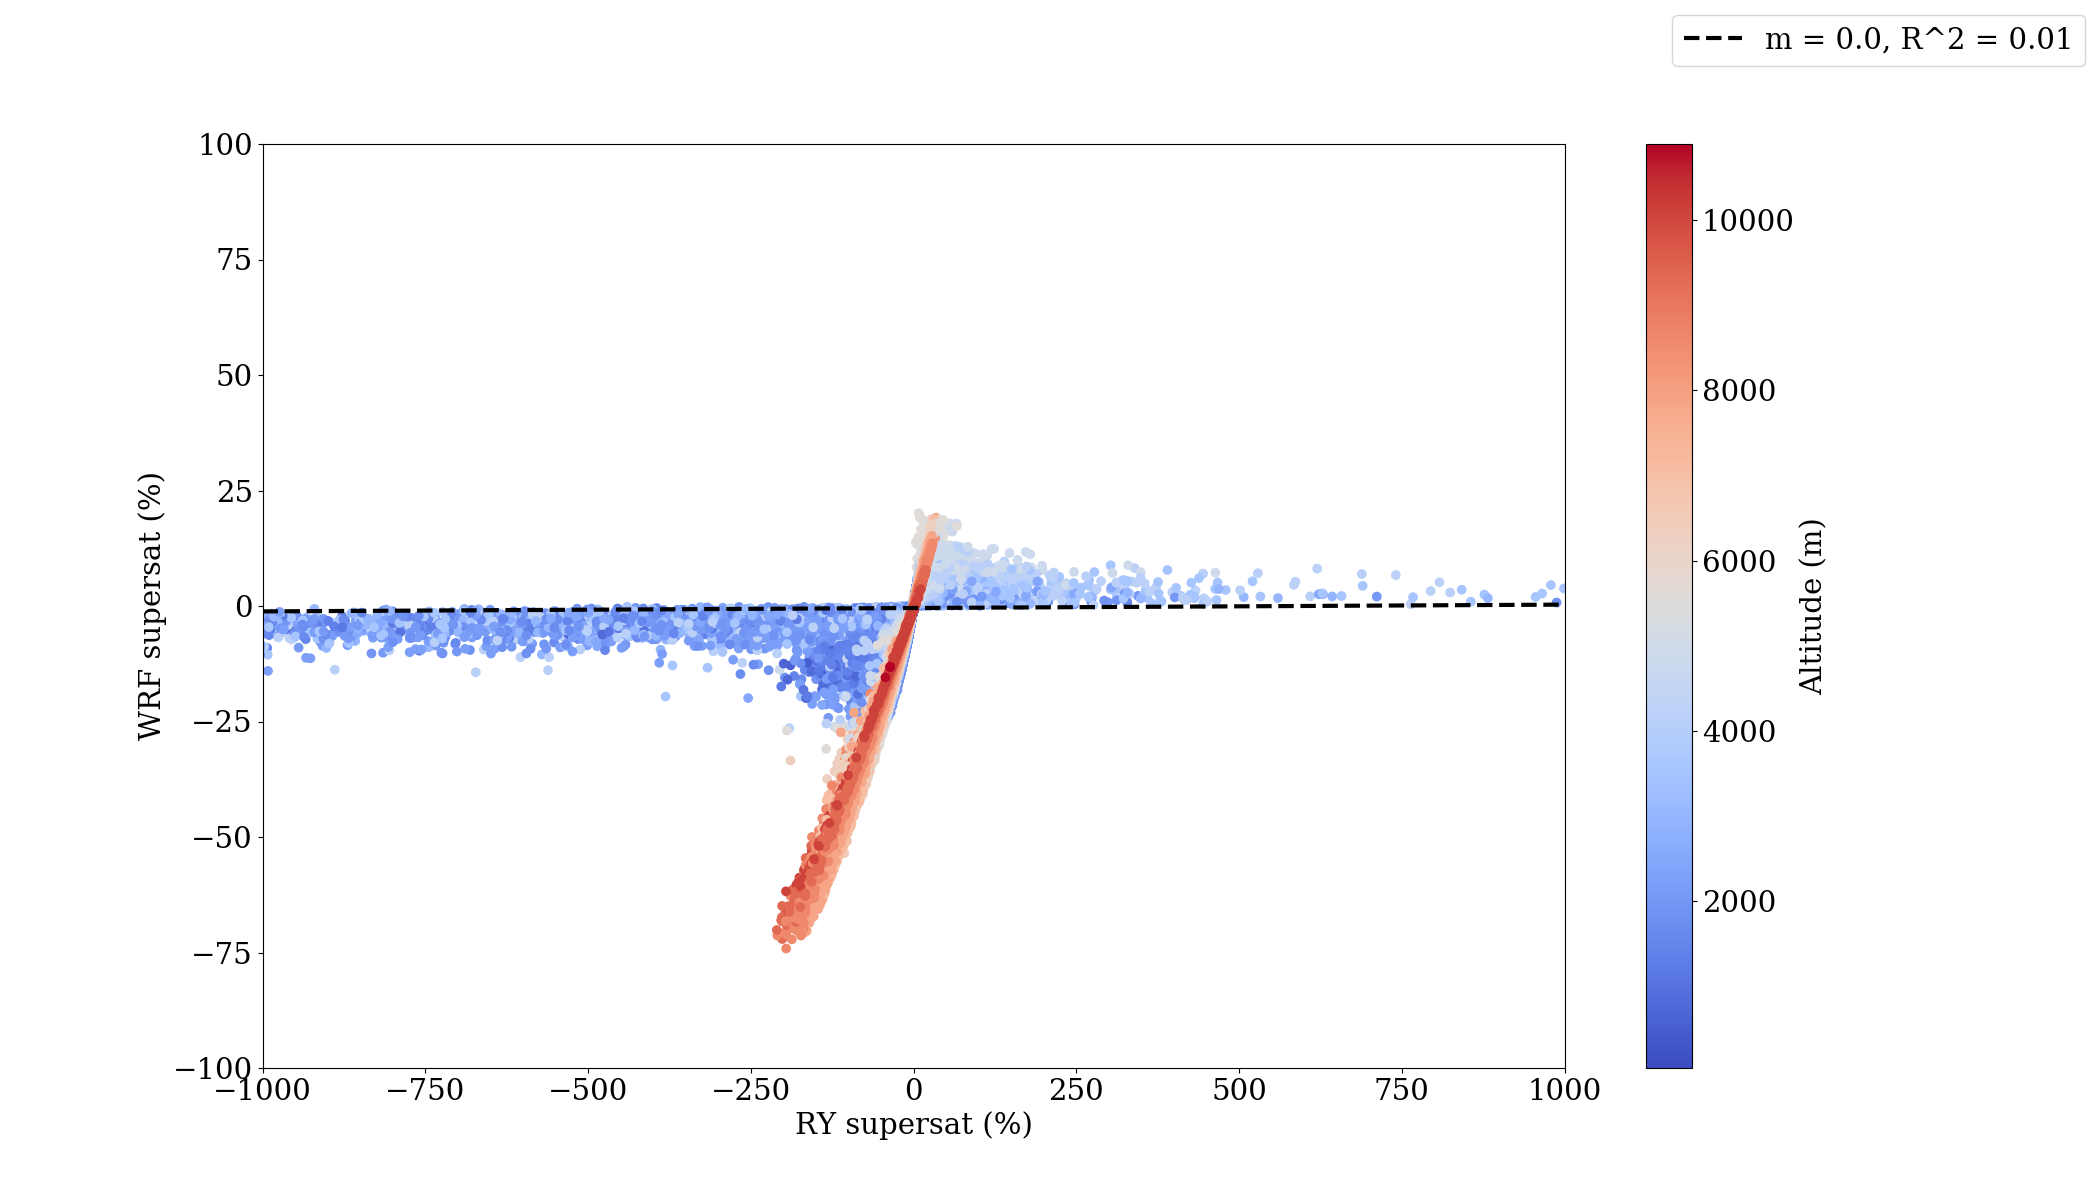
\includegraphics[width=10cm]{mywrf/v37_backtrack_qss_Polluted_figure.png}
    \caption{$SS_{RY}$ as described by Equation (\ref{ssry}) vs WRF SS output, polluted case. Points plotted have LWC $> 10^{-5}$. The domain has been restricted manually.}
    \label{v37pol}
\end{figure}

\begin{figure}[h]
    \centering
    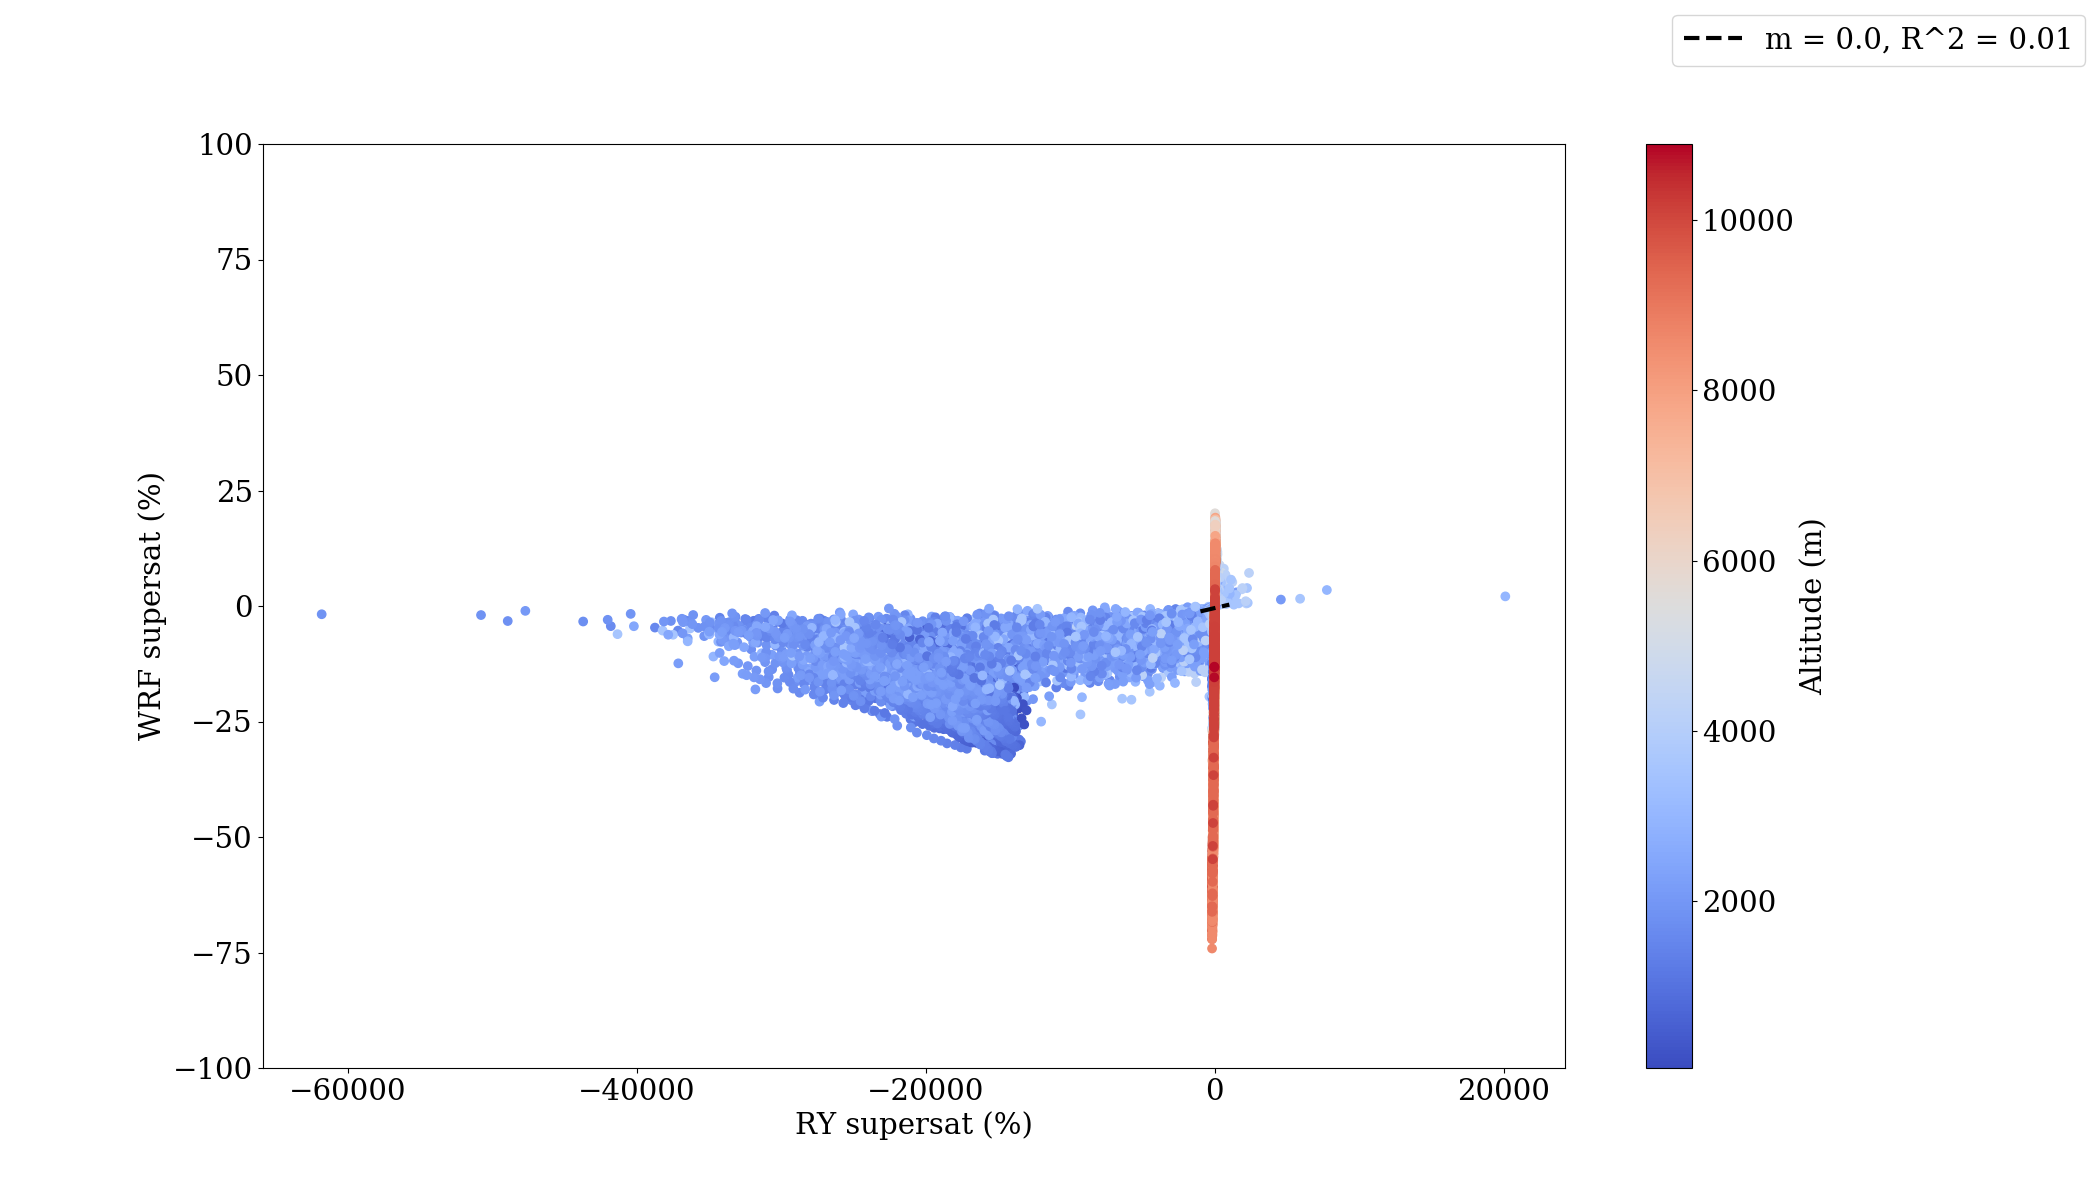
\includegraphics[width=10cm]{mywrf/v38_backtrack_qss_Polluted_figure.png}
    \caption{Same as Figure (\ref{v37pol}), but with the full domain.}
    \label{v38pol}
\end{figure}

\begin{figure}[h]
    \centering
    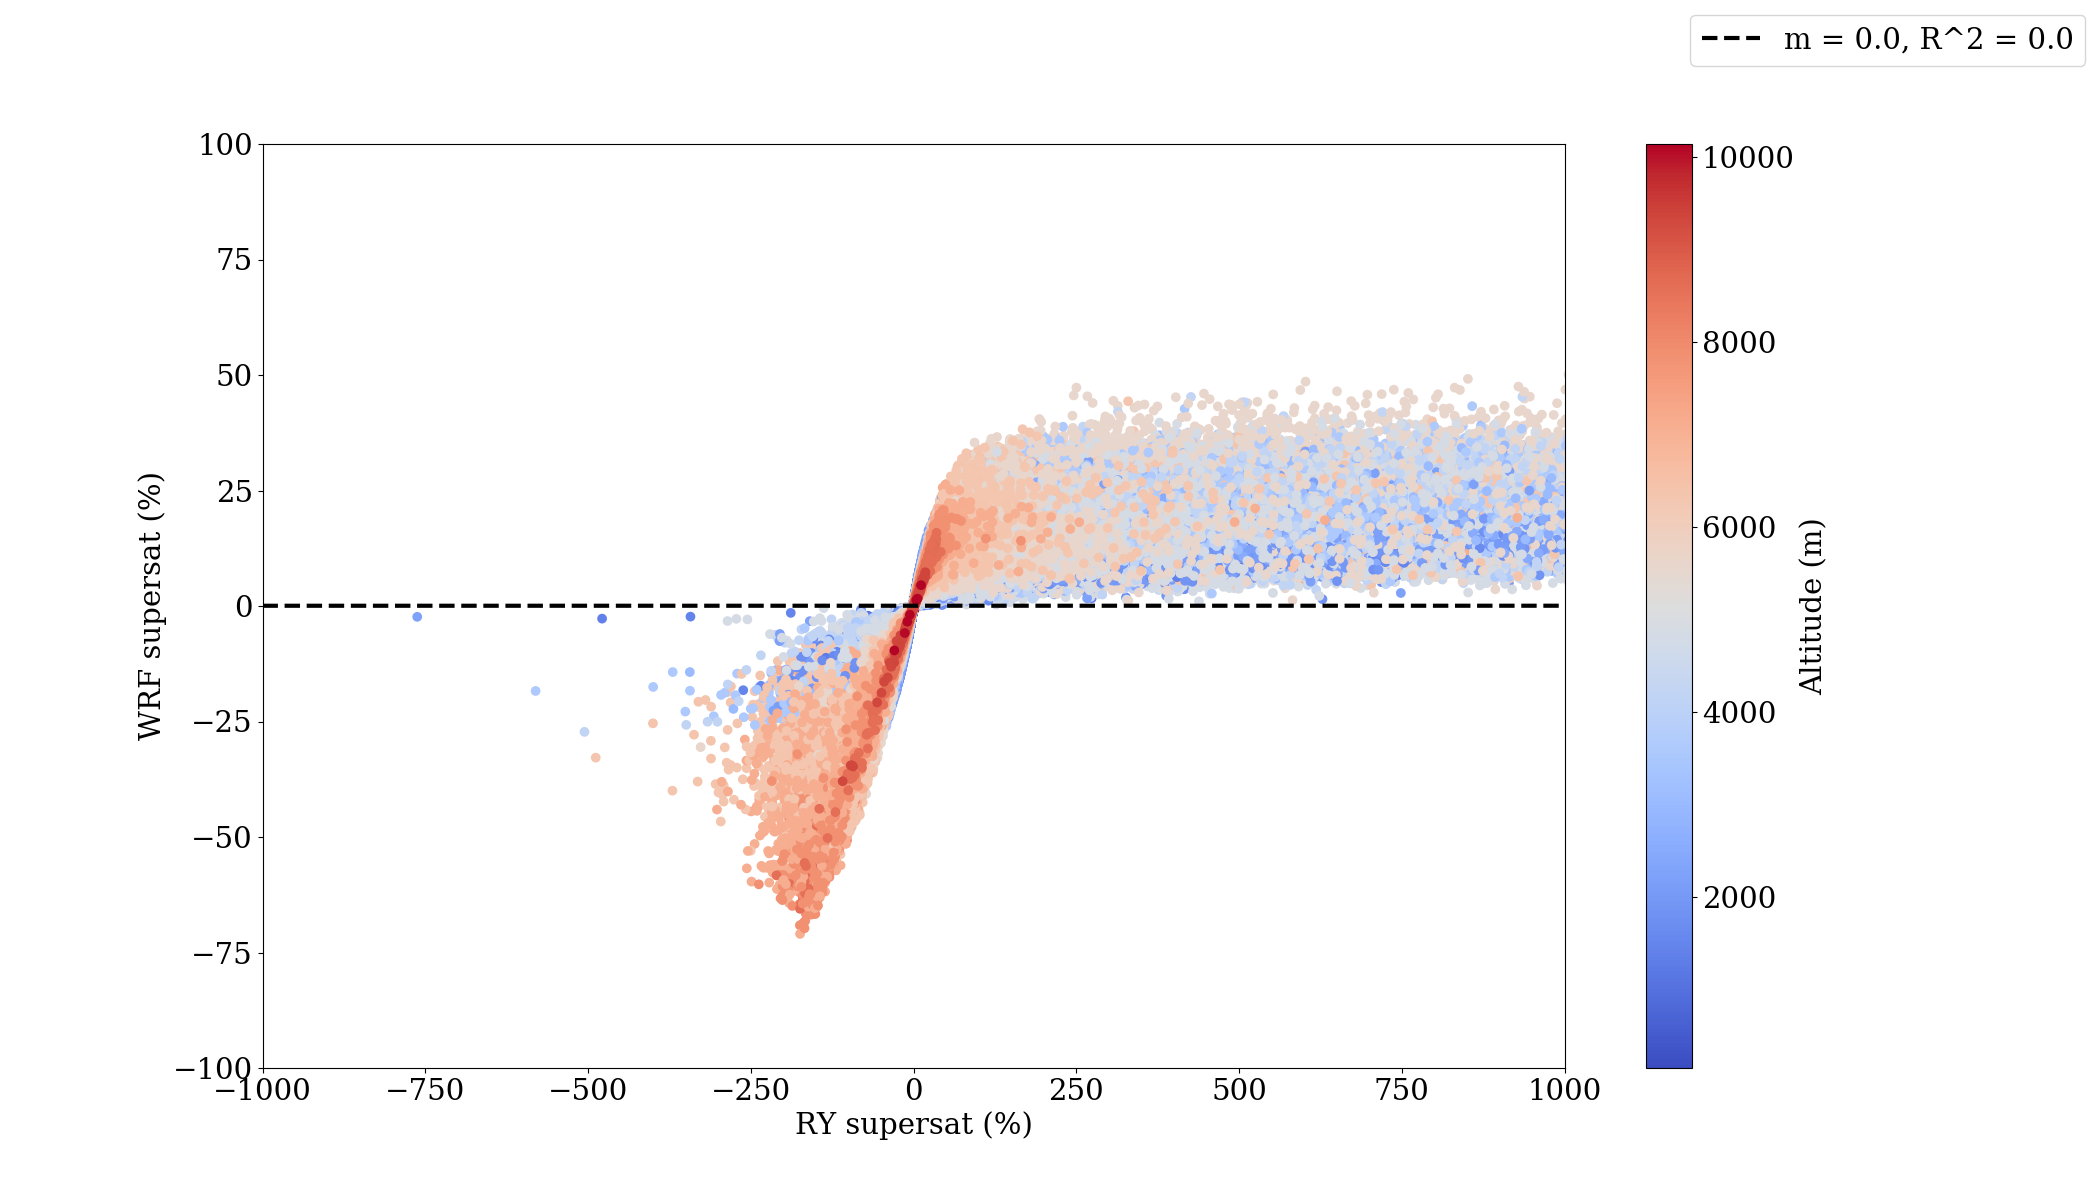
\includegraphics[width=10cm]{mywrf/v37_backtrack_qss_Unpolluted_figure.png}
    \caption{$SS_{RY}$ as described by Equation (\ref{ssry}) vs WRF SS output, unpolluted case. Points plotted have LWC $> 10^{-5}$. The domain has been restricted manually.}
    \label{v37unpol}
\end{figure}

\begin{figure}[h]
    \centering
    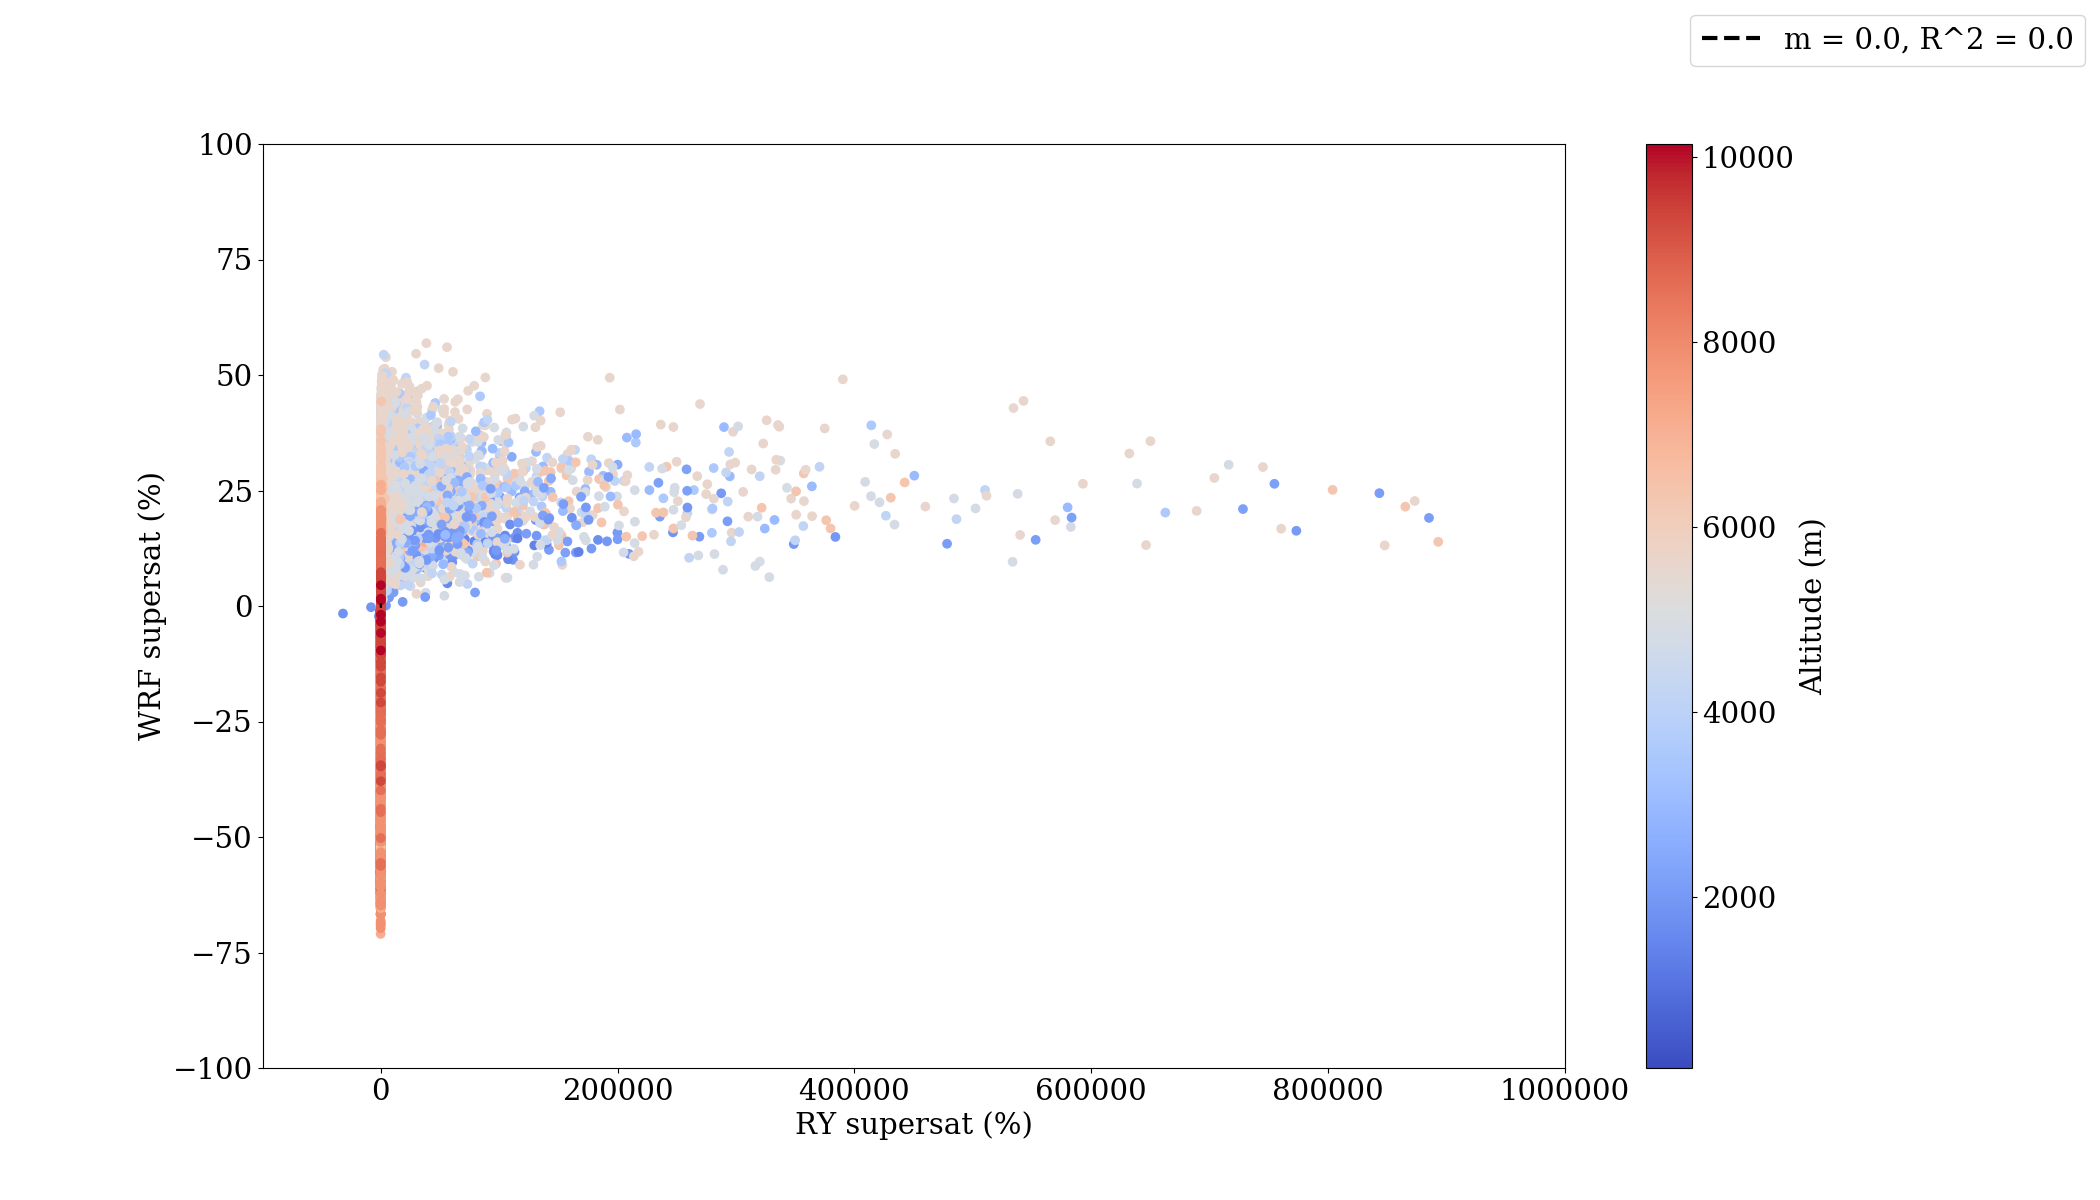
\includegraphics[width=10cm]{mywrf/v38_backtrack_qss_Unpolluted_figure.png}
    \caption{Same as Figure (\ref{v37unpol}), but with the full domain.}
    \label{v38unpol}
\end{figure}

\clearpage

Can disagreement be attributed to neglect of finite droplet size effects? We would expect those effects to occur in cases where mean radius is smallest. However it seems this would not explain what we are seeing in Figures (\ref{v37pol})-(\ref{v38unpol}):

\begin{figure}[h]
    \centering
    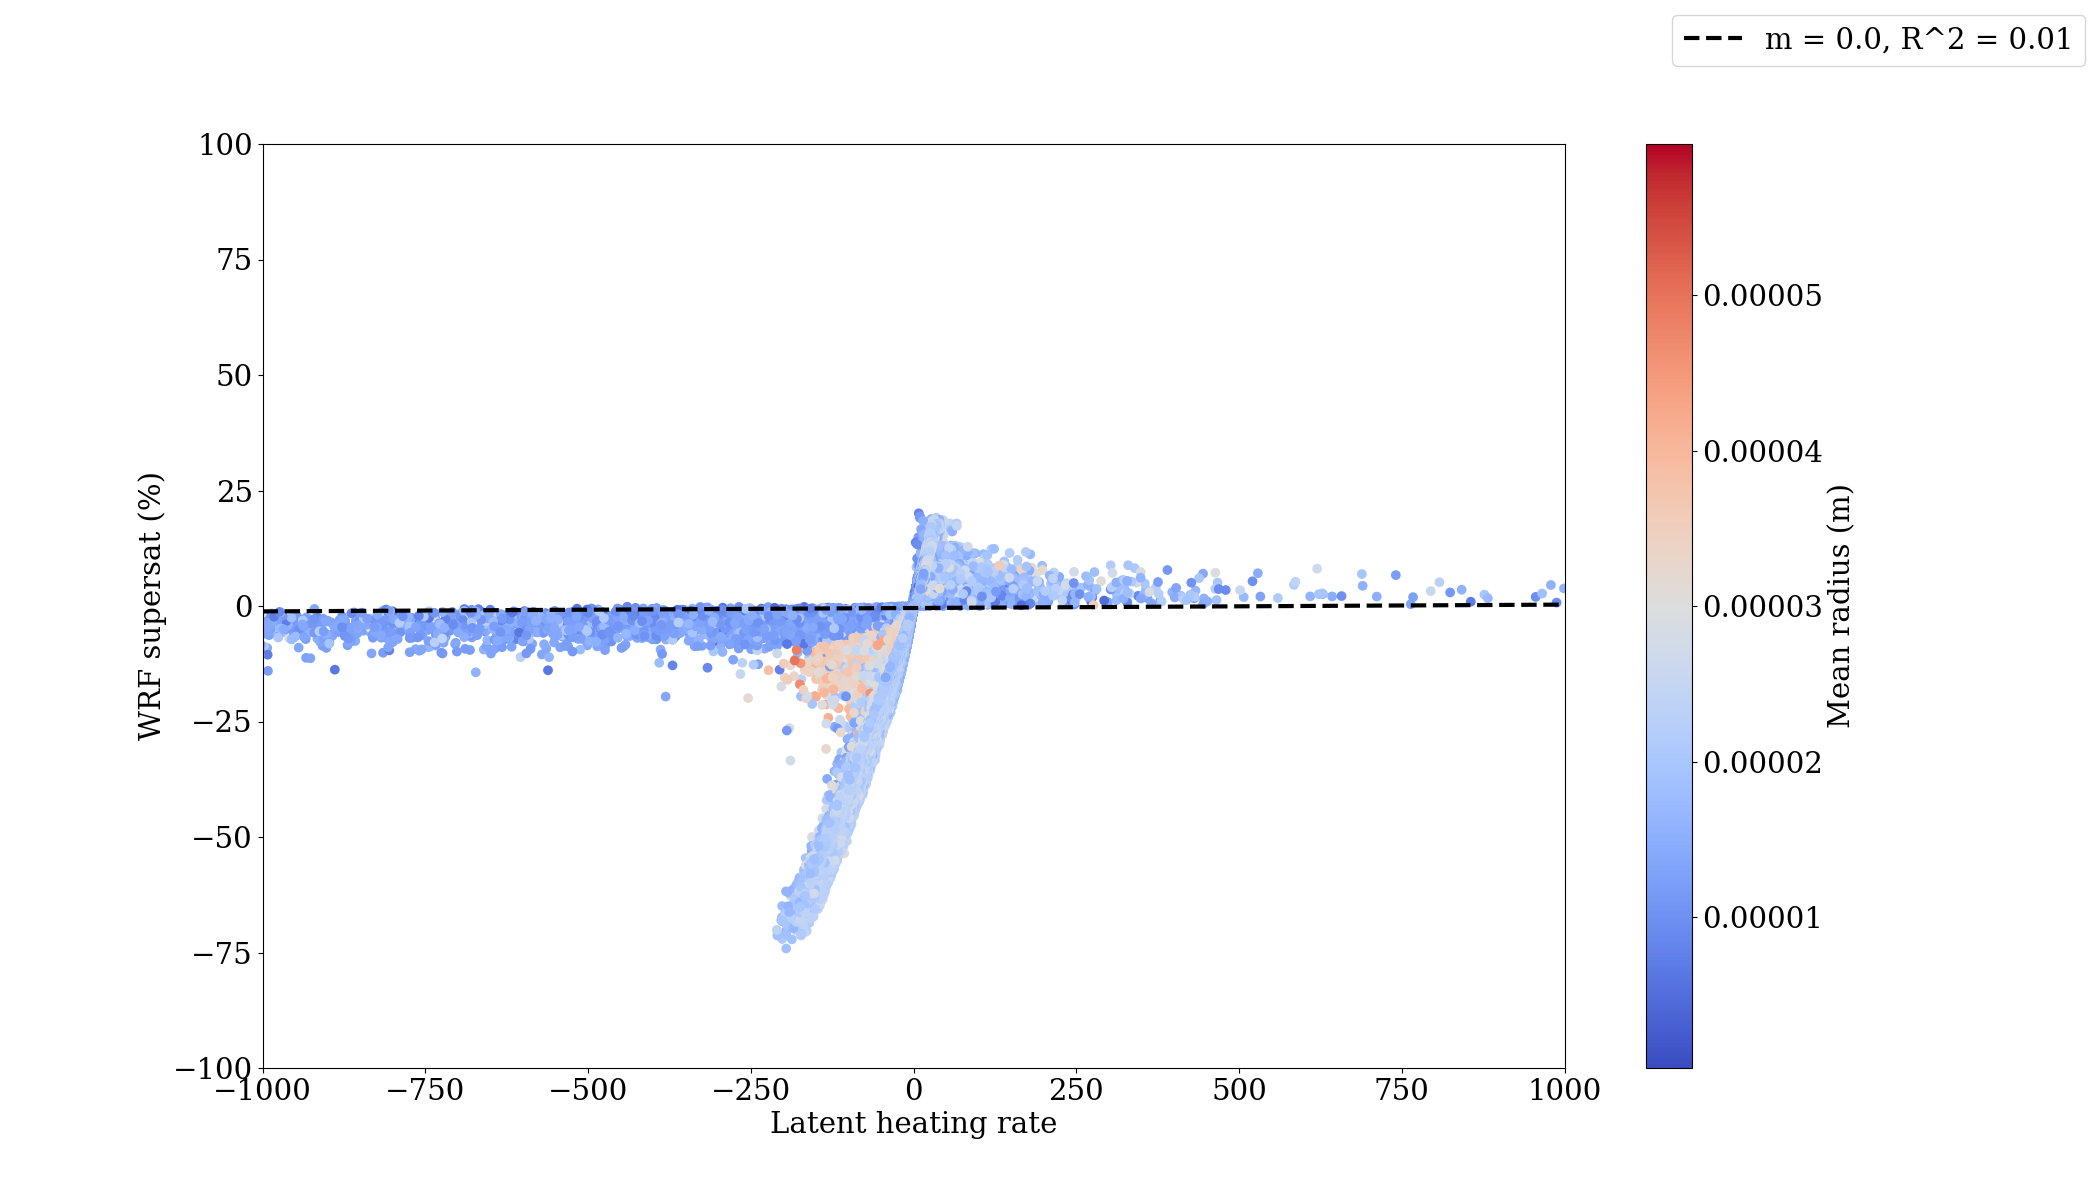
\includegraphics[width=10cm]{mywrf/v19_backtrack_qss_Polluted_figure.png}
    \caption{$SS_{RY}$ as described by Equation (\ref{ssry}) vs WRF SS output, polluted case. Points plotted have LWC $> 10^{-5}$. The domain has been restricted manually.}
    \label{v19pol}
\end{figure}

\begin{figure}[h]
    \centering
    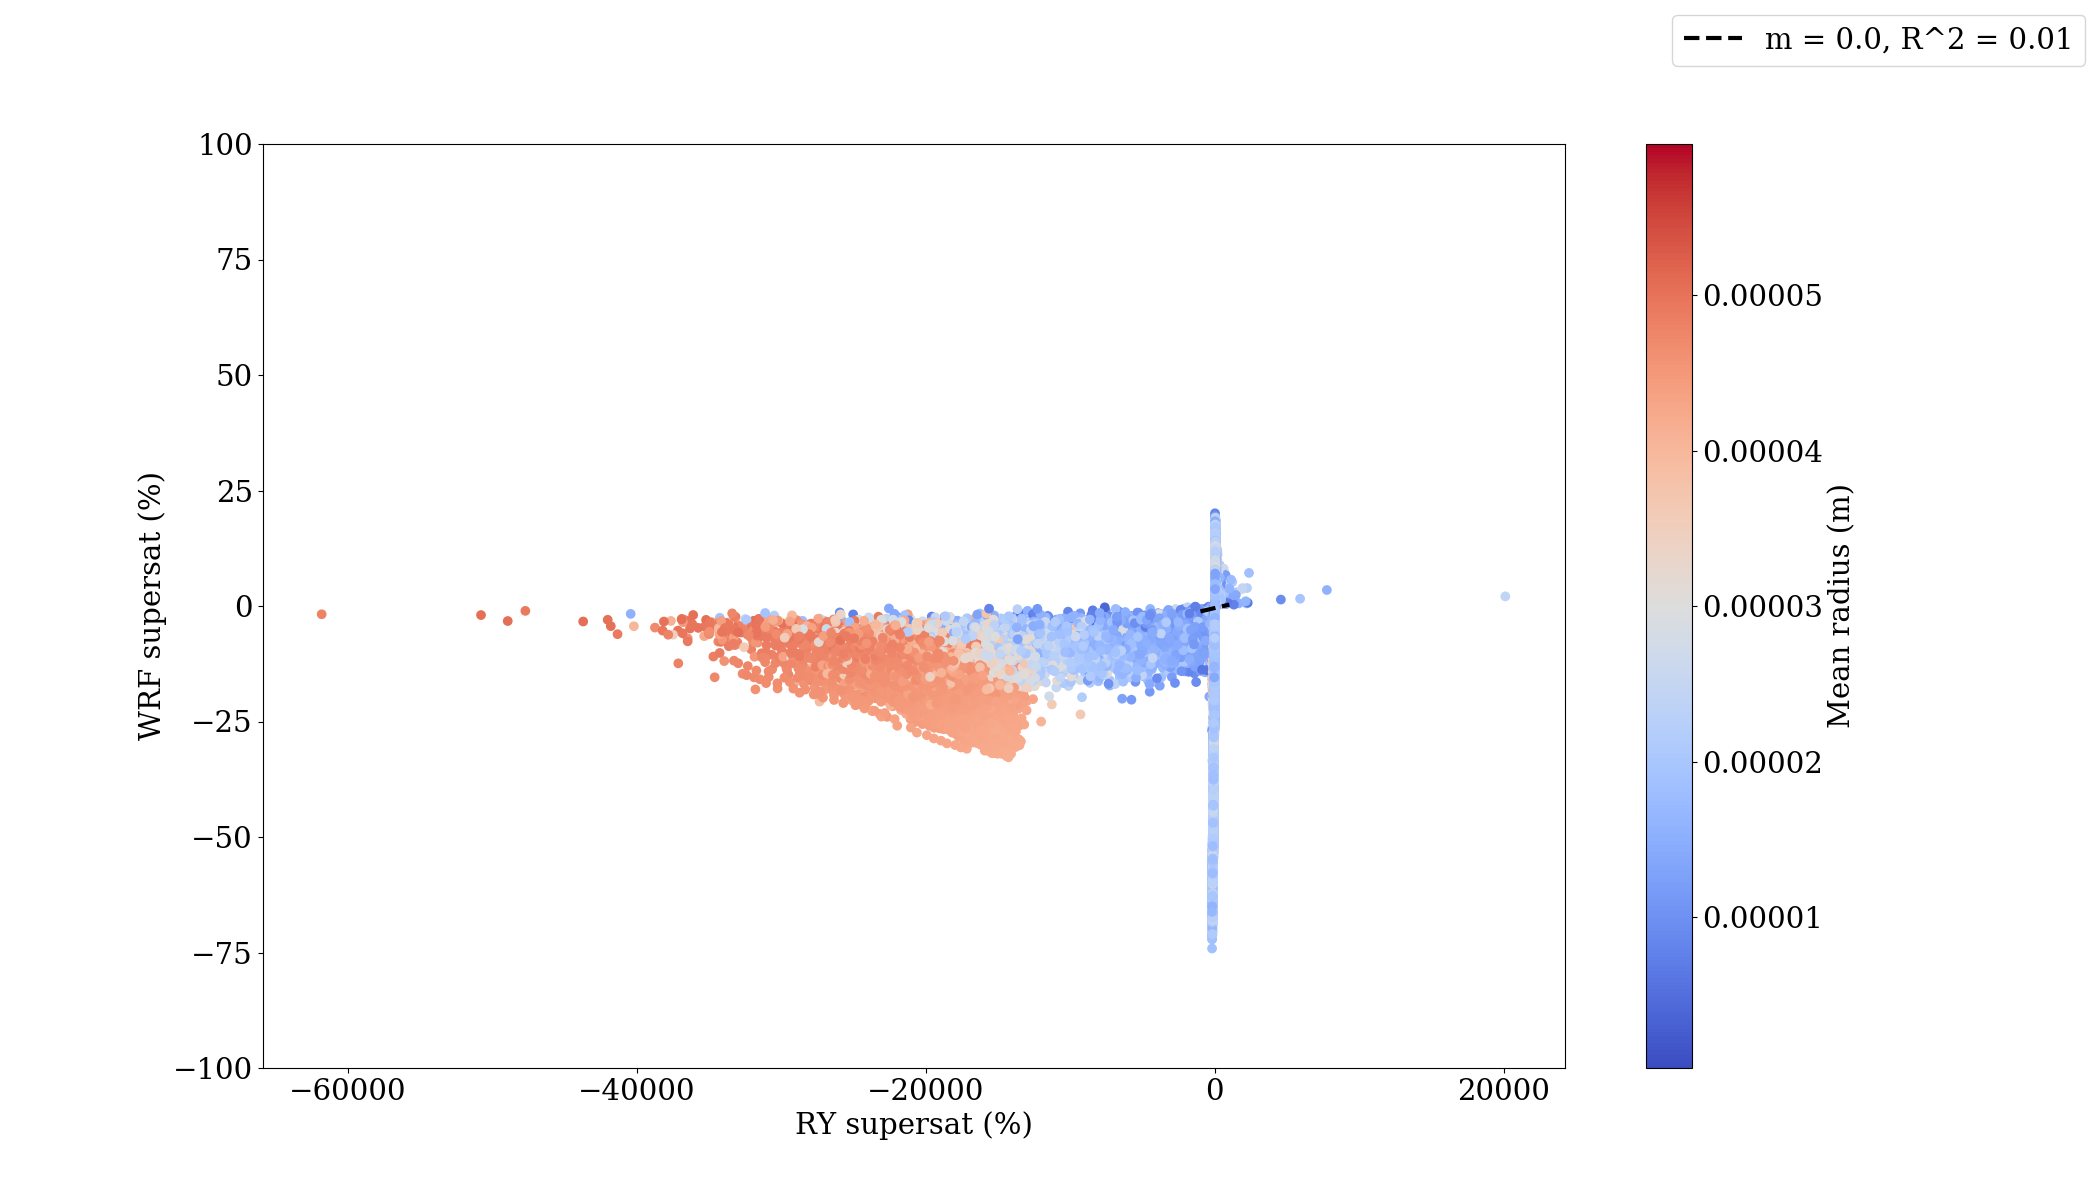
\includegraphics[width=10cm]{mywrf/v20_backtrack_qss_Polluted_figure.png}
    \caption{Same as Figure (\ref{v19pol}), but with the full domain.}
    \label{v20pol}
\end{figure}

\begin{figure}[h]
    \centering
    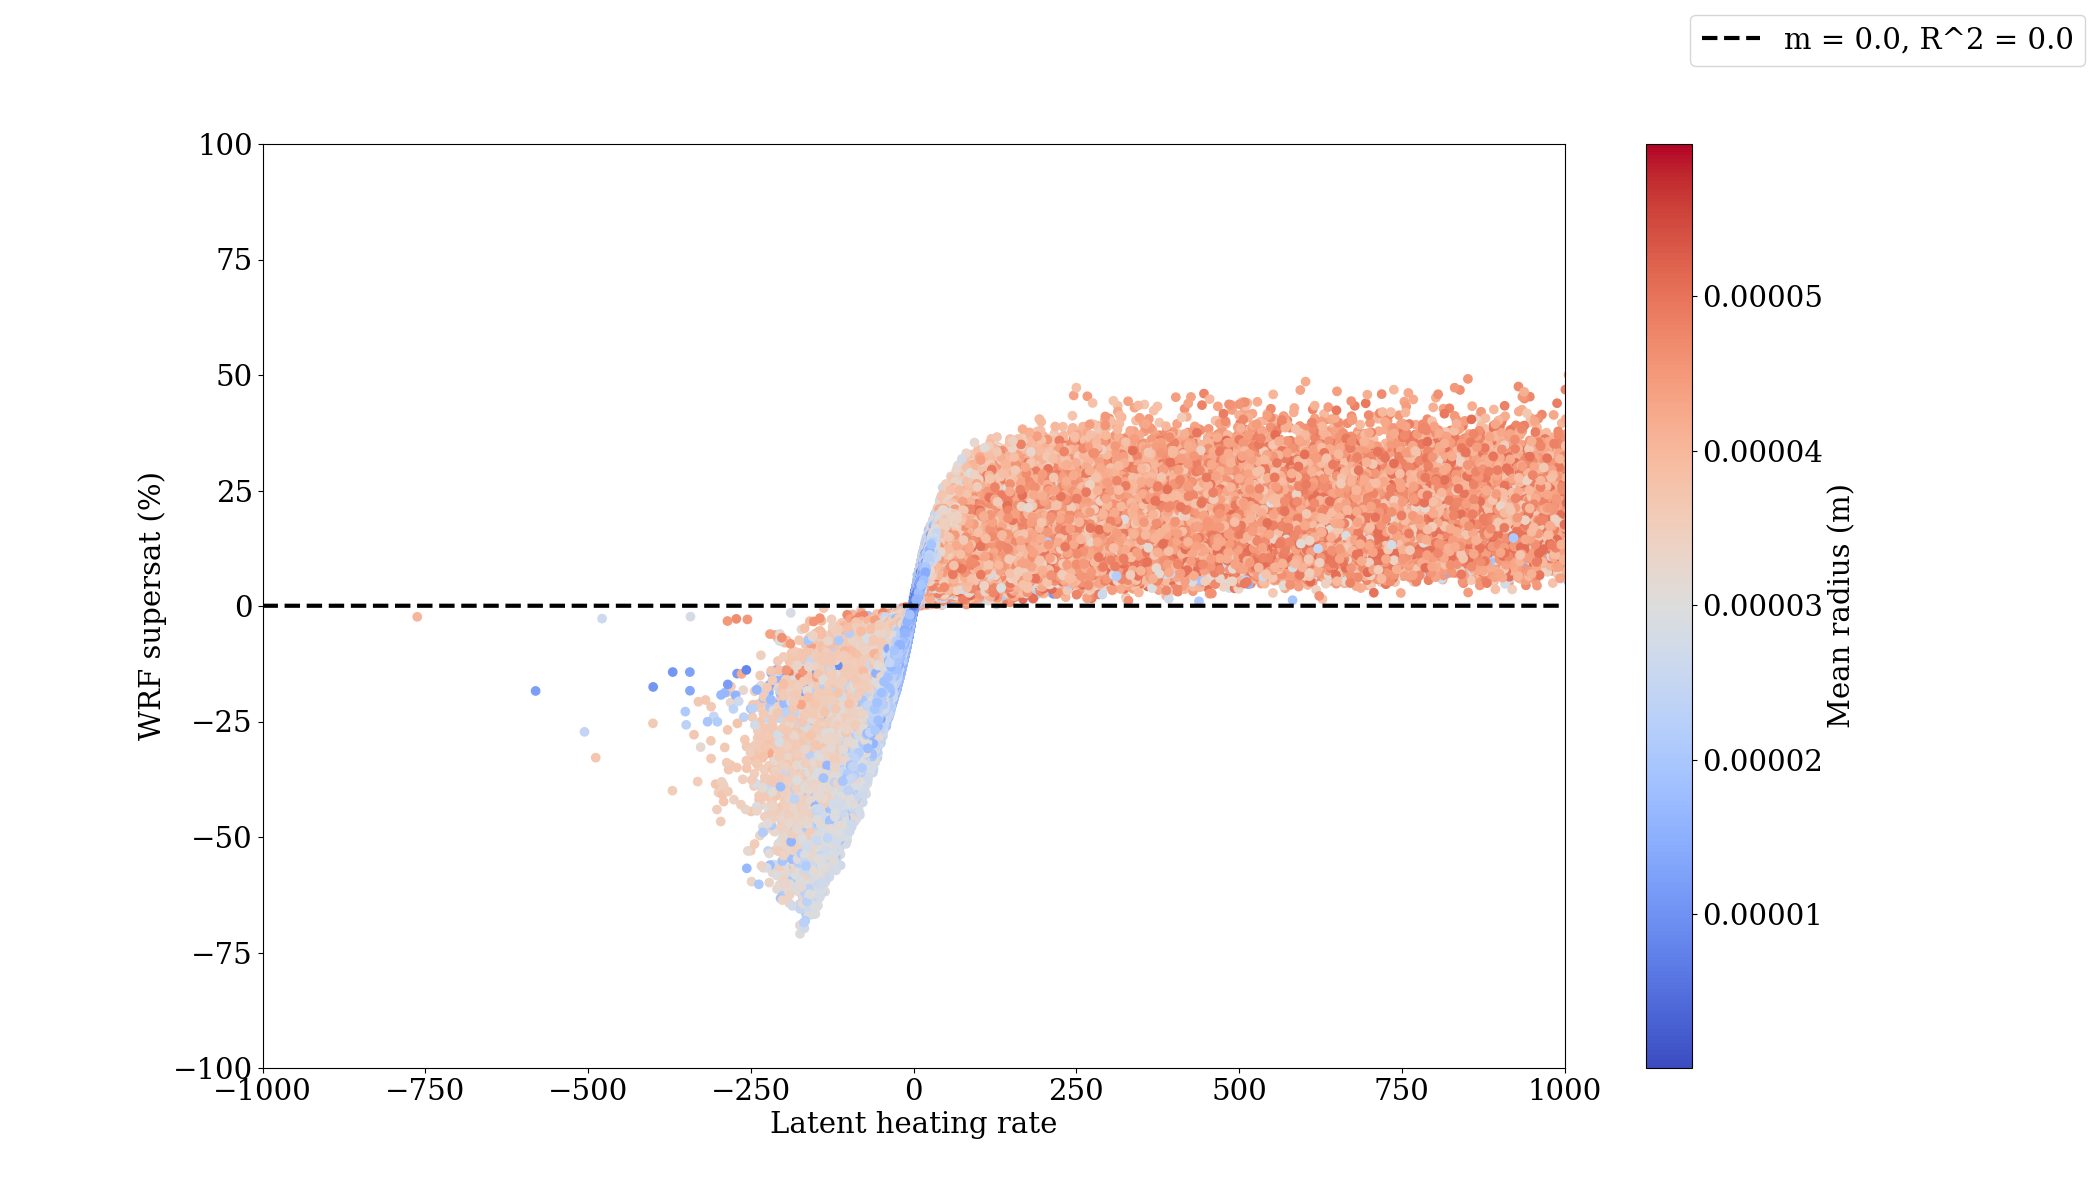
\includegraphics[width=10cm]{mywrf/v19_backtrack_qss_Unpolluted_figure.png}
    \caption{$SS_{RY}$ as described by Equation (\ref{ssry}) vs WRF SS output, unpolluted case. Points plotted have LWC $> 10^{-5}$. The domain has been restricted manually.}
    \label{v19unpol}
\end{figure}

\begin{figure}[h]
    \centering
    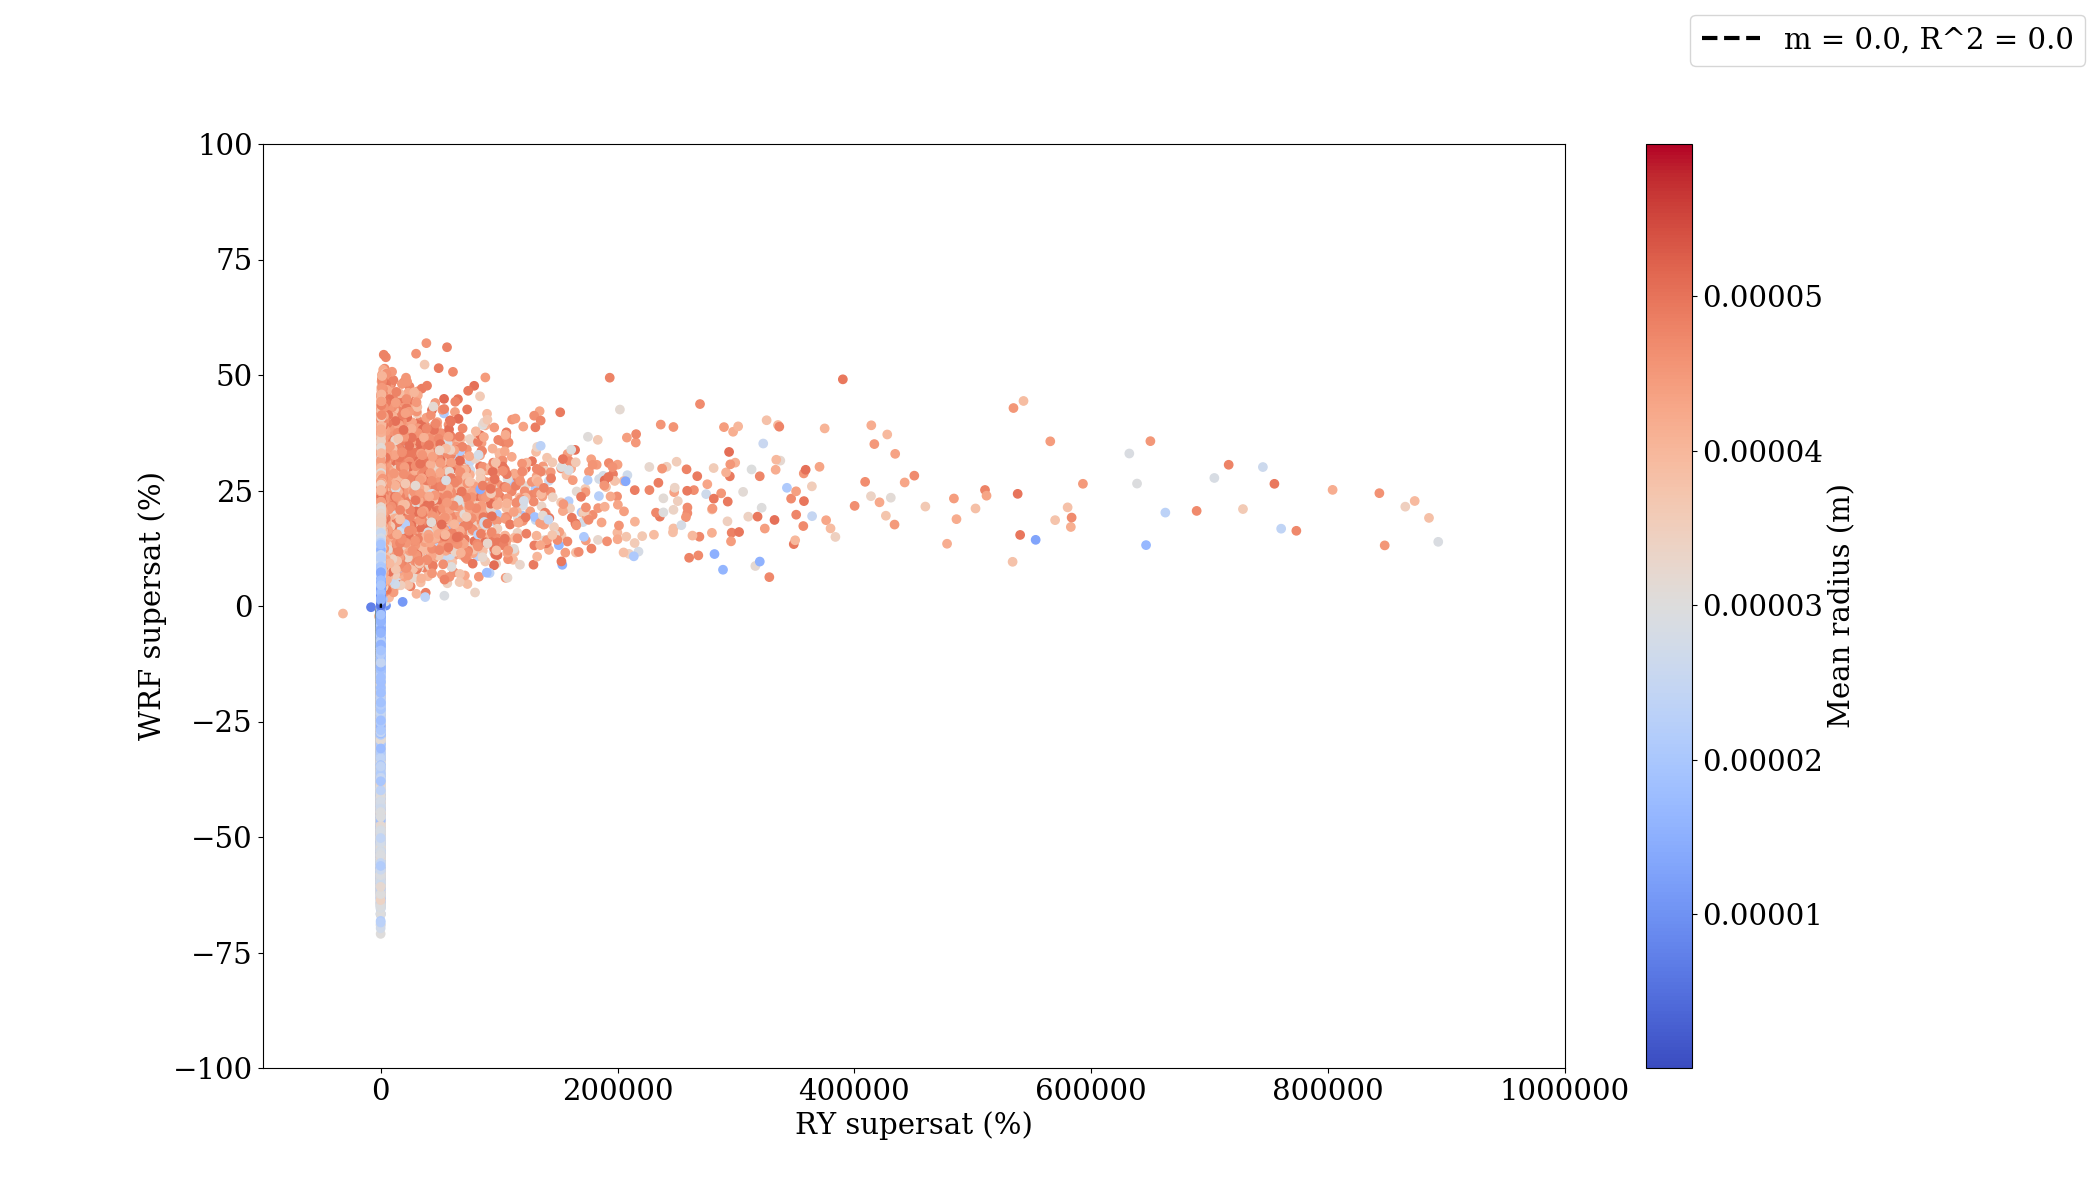
\includegraphics[width=10cm]{mywrf/v20_backtrack_qss_Unpolluted_figure.png}
    \caption{Same as Figure (\ref{v19unpol}), but with the full domain.}
    \label{v20unpol}
\end{figure}

\clearpage

Increasing the LWC cutoff does seem to improve the situation, however (see figures below). Based on my own exploration this has a similar effect to filtering out low-$n$ points (unsurprising then that many of the large-$SS_{RY}$ points are removed, since $n$ appears in the denominator).

\begin{figure}[h]
    \centering
    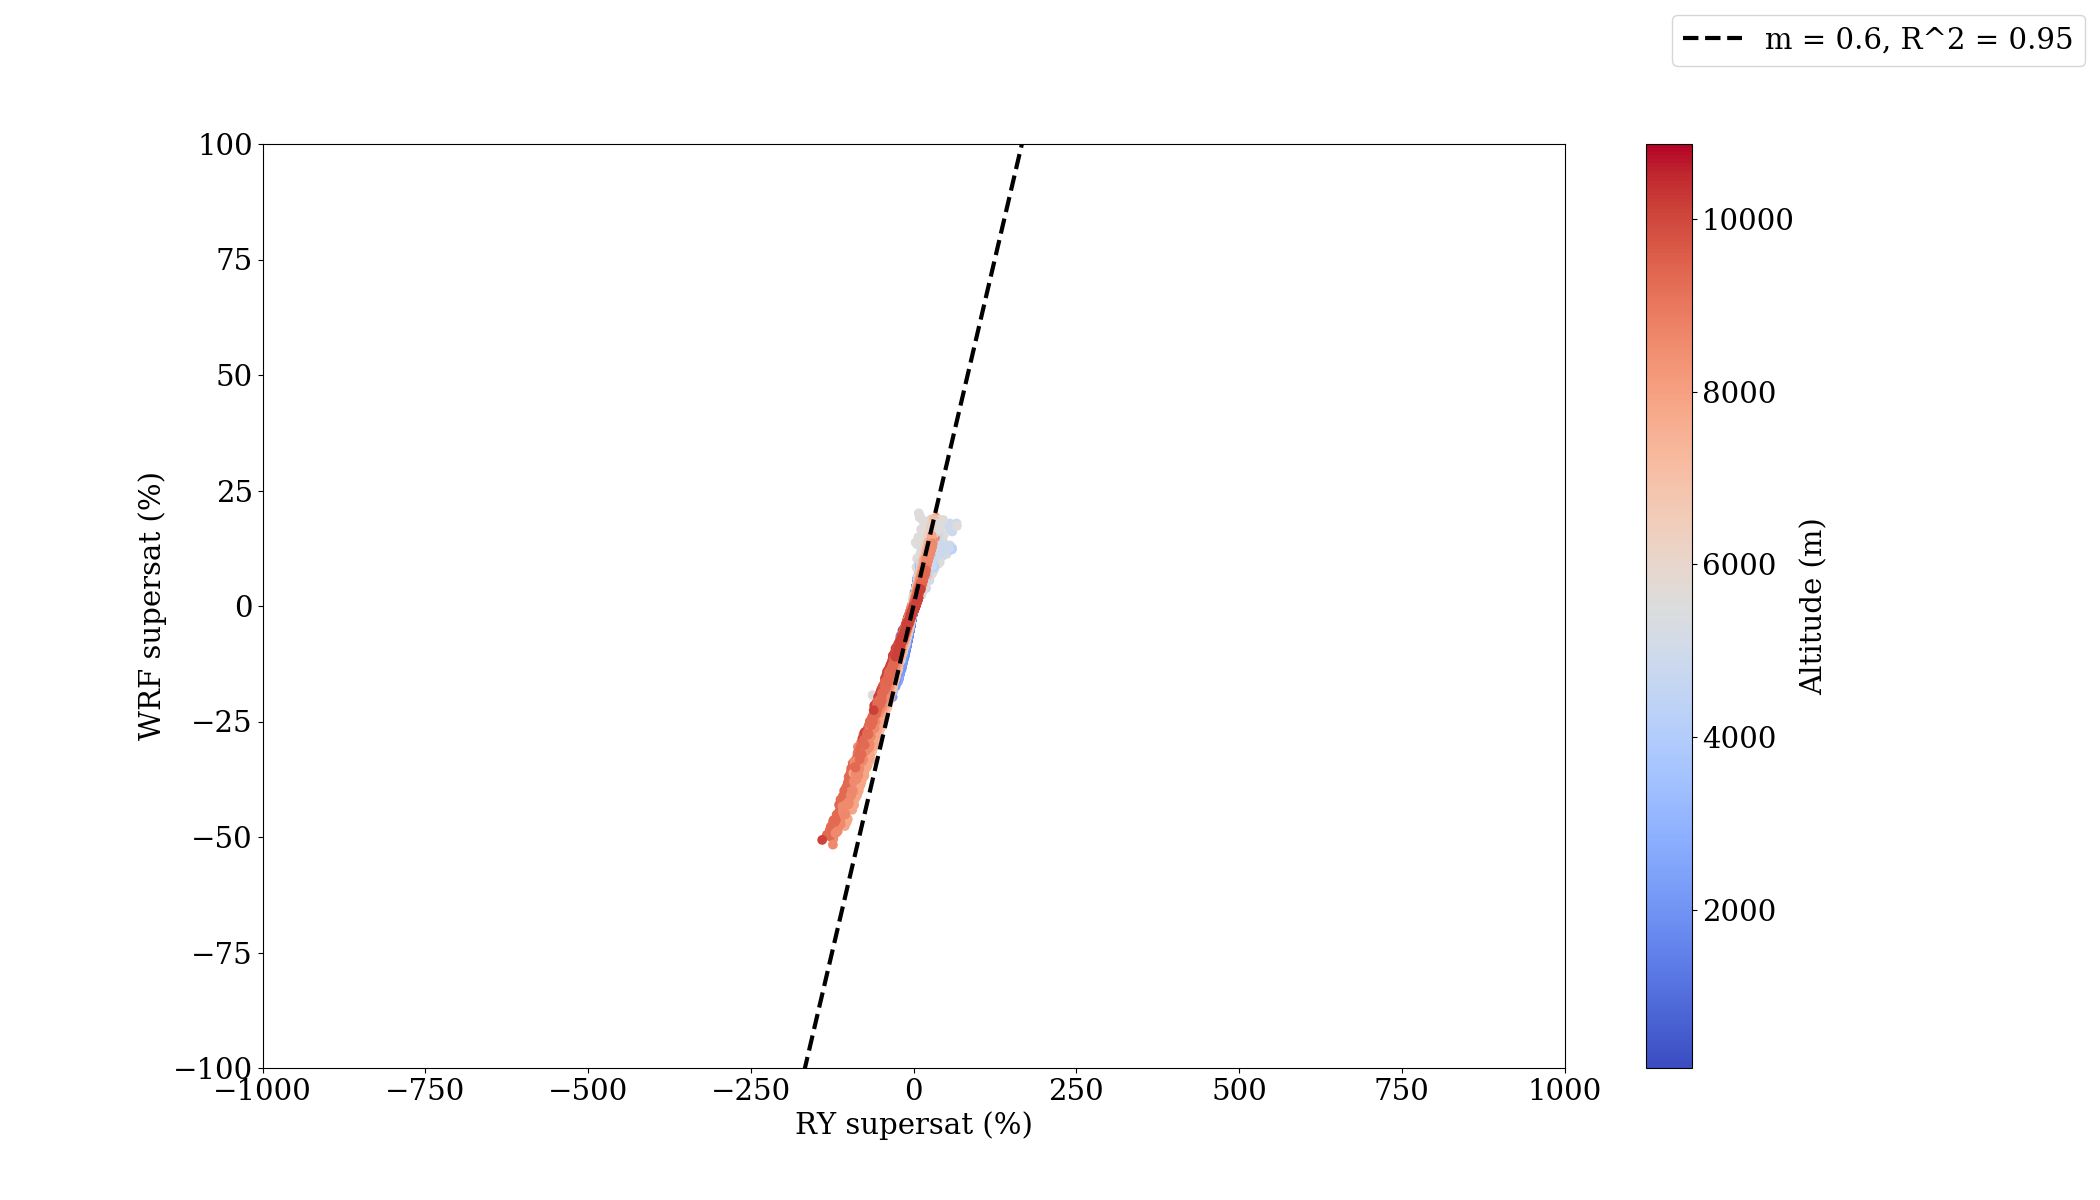
\includegraphics[width=10cm]{mywrf/v39_backtrack_qss_Polluted_figure.png}
    \caption{$SS_{RY}$ as described by Equation (\ref{ssry}) vs WRF SS output, polluted case. Points plotted have LWC $> 5*10^{-5}$. The domain has been restricted manually.}
    \label{v39pol}
\end{figure}

\begin{figure}[h]
    \centering
    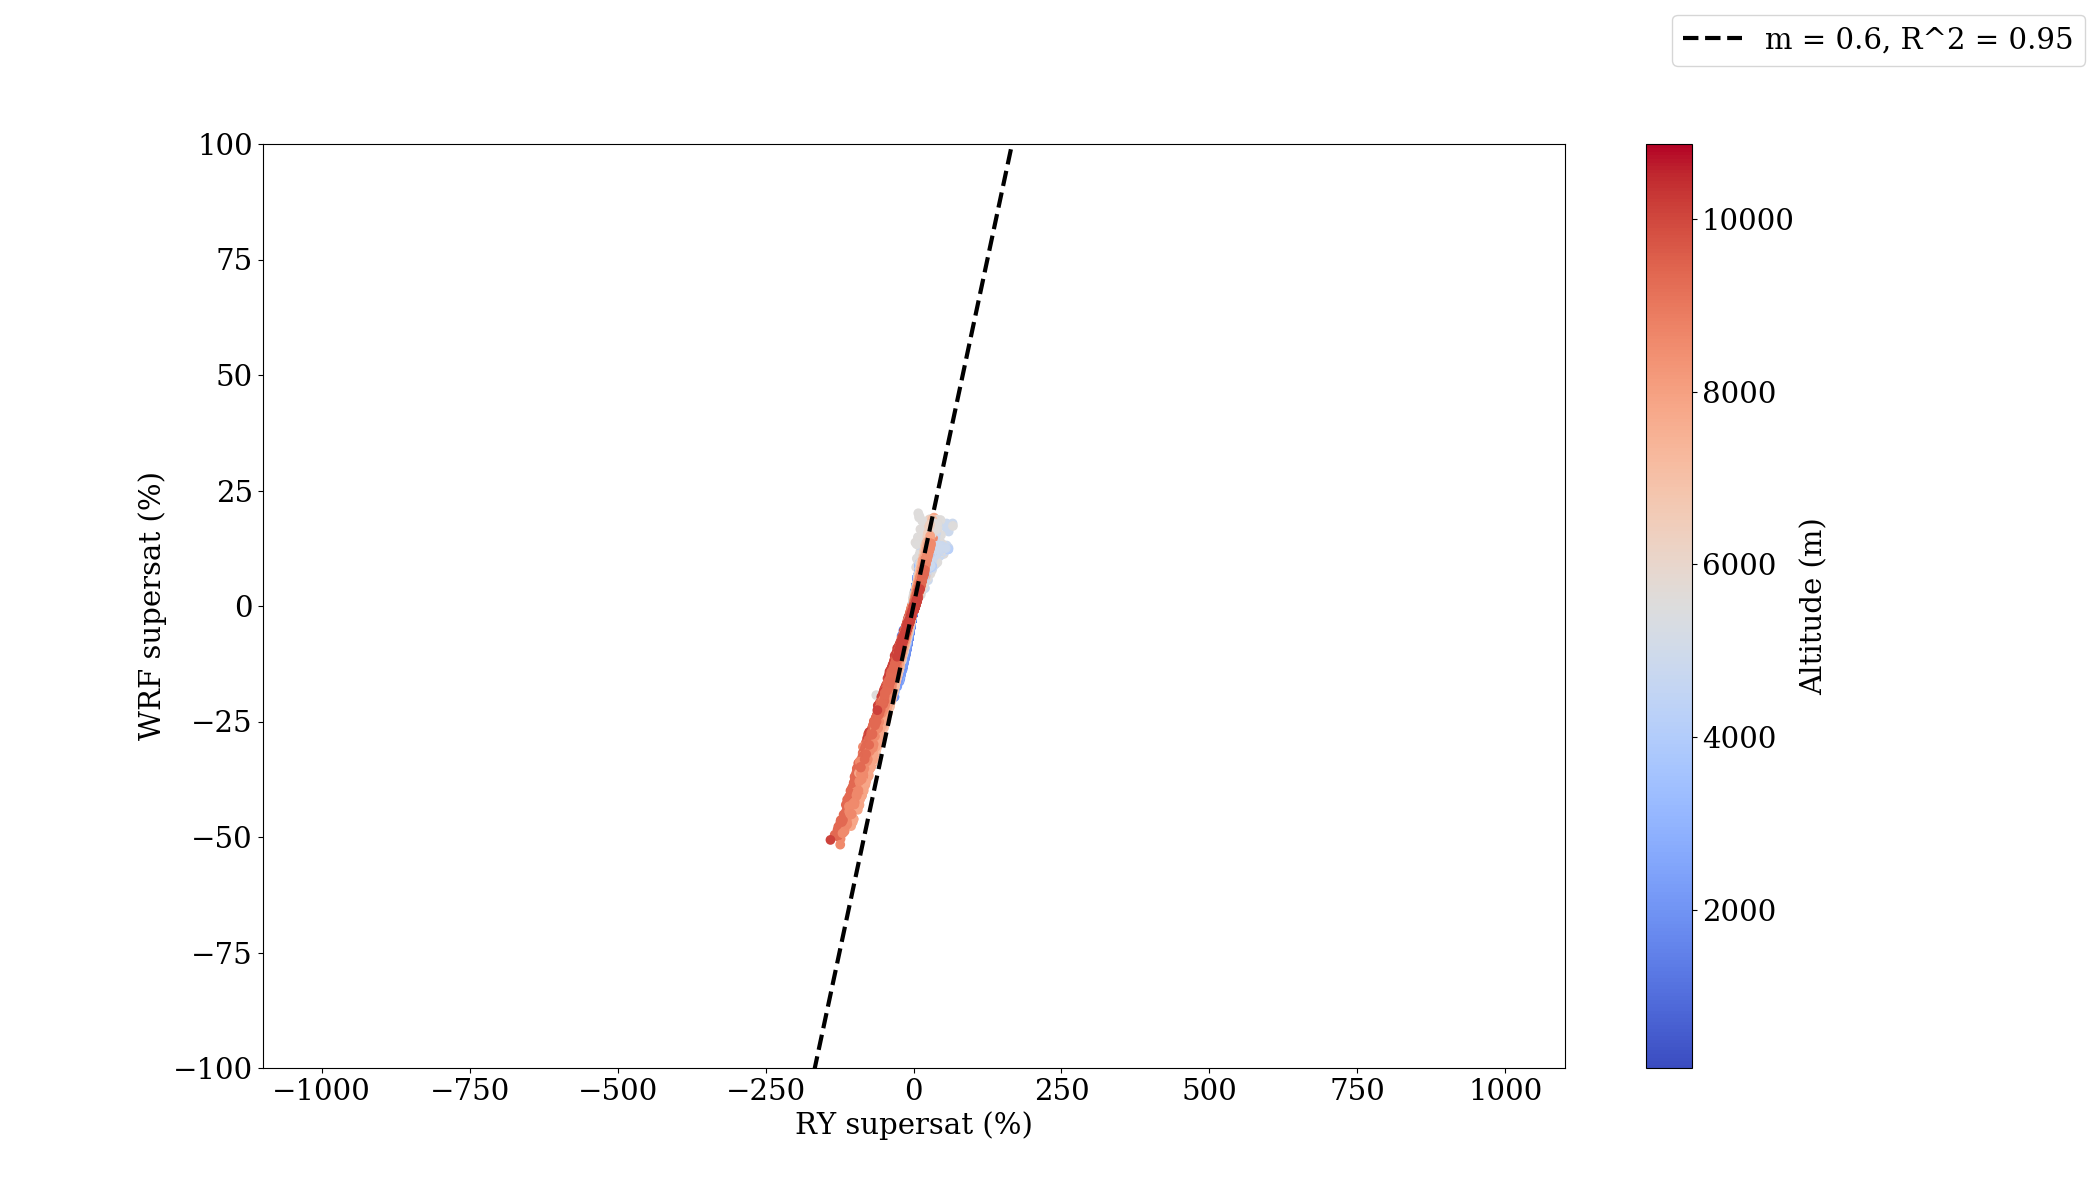
\includegraphics[width=10cm]{mywrf/v40_backtrack_qss_Polluted_figure.png}
    \caption{Same as Figure (\ref{v39pol}), but with the full domain.}
    \label{v40pol}
\end{figure}

\begin{figure}[h]
    \centering
    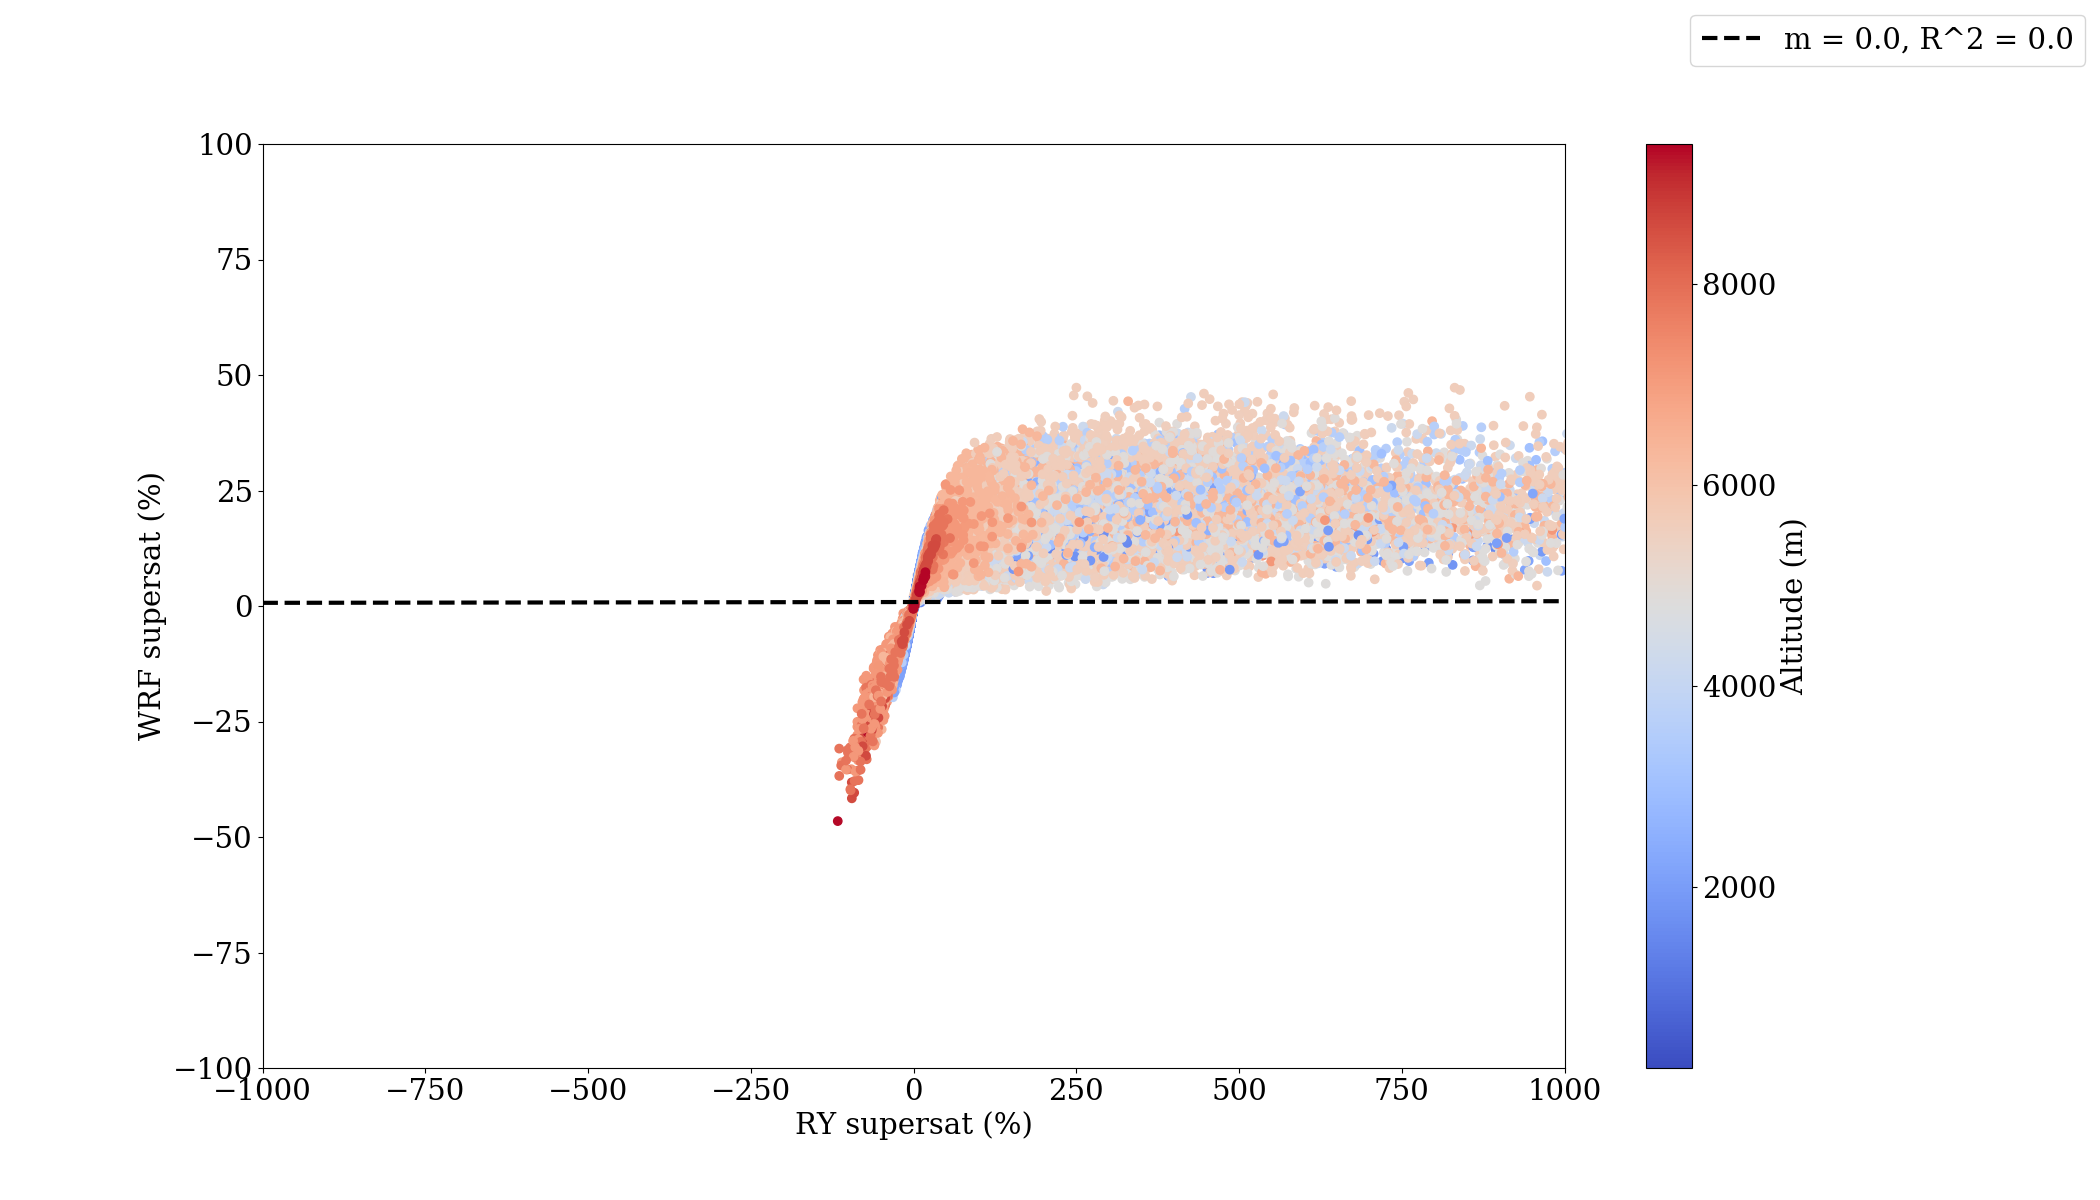
\includegraphics[width=10cm]{mywrf/v39_backtrack_qss_Unpolluted_figure.png}
    \caption{$SS_{RY}$ as described by Equation (\ref{ssry}) vs WRF SS output, unpolluted case. Points plotted have LWC $> 5*10^{-5}$. The domain has been restricted manually.}
    \label{v39unpol}
\end{figure}

\begin{figure}[h]
    \centering
    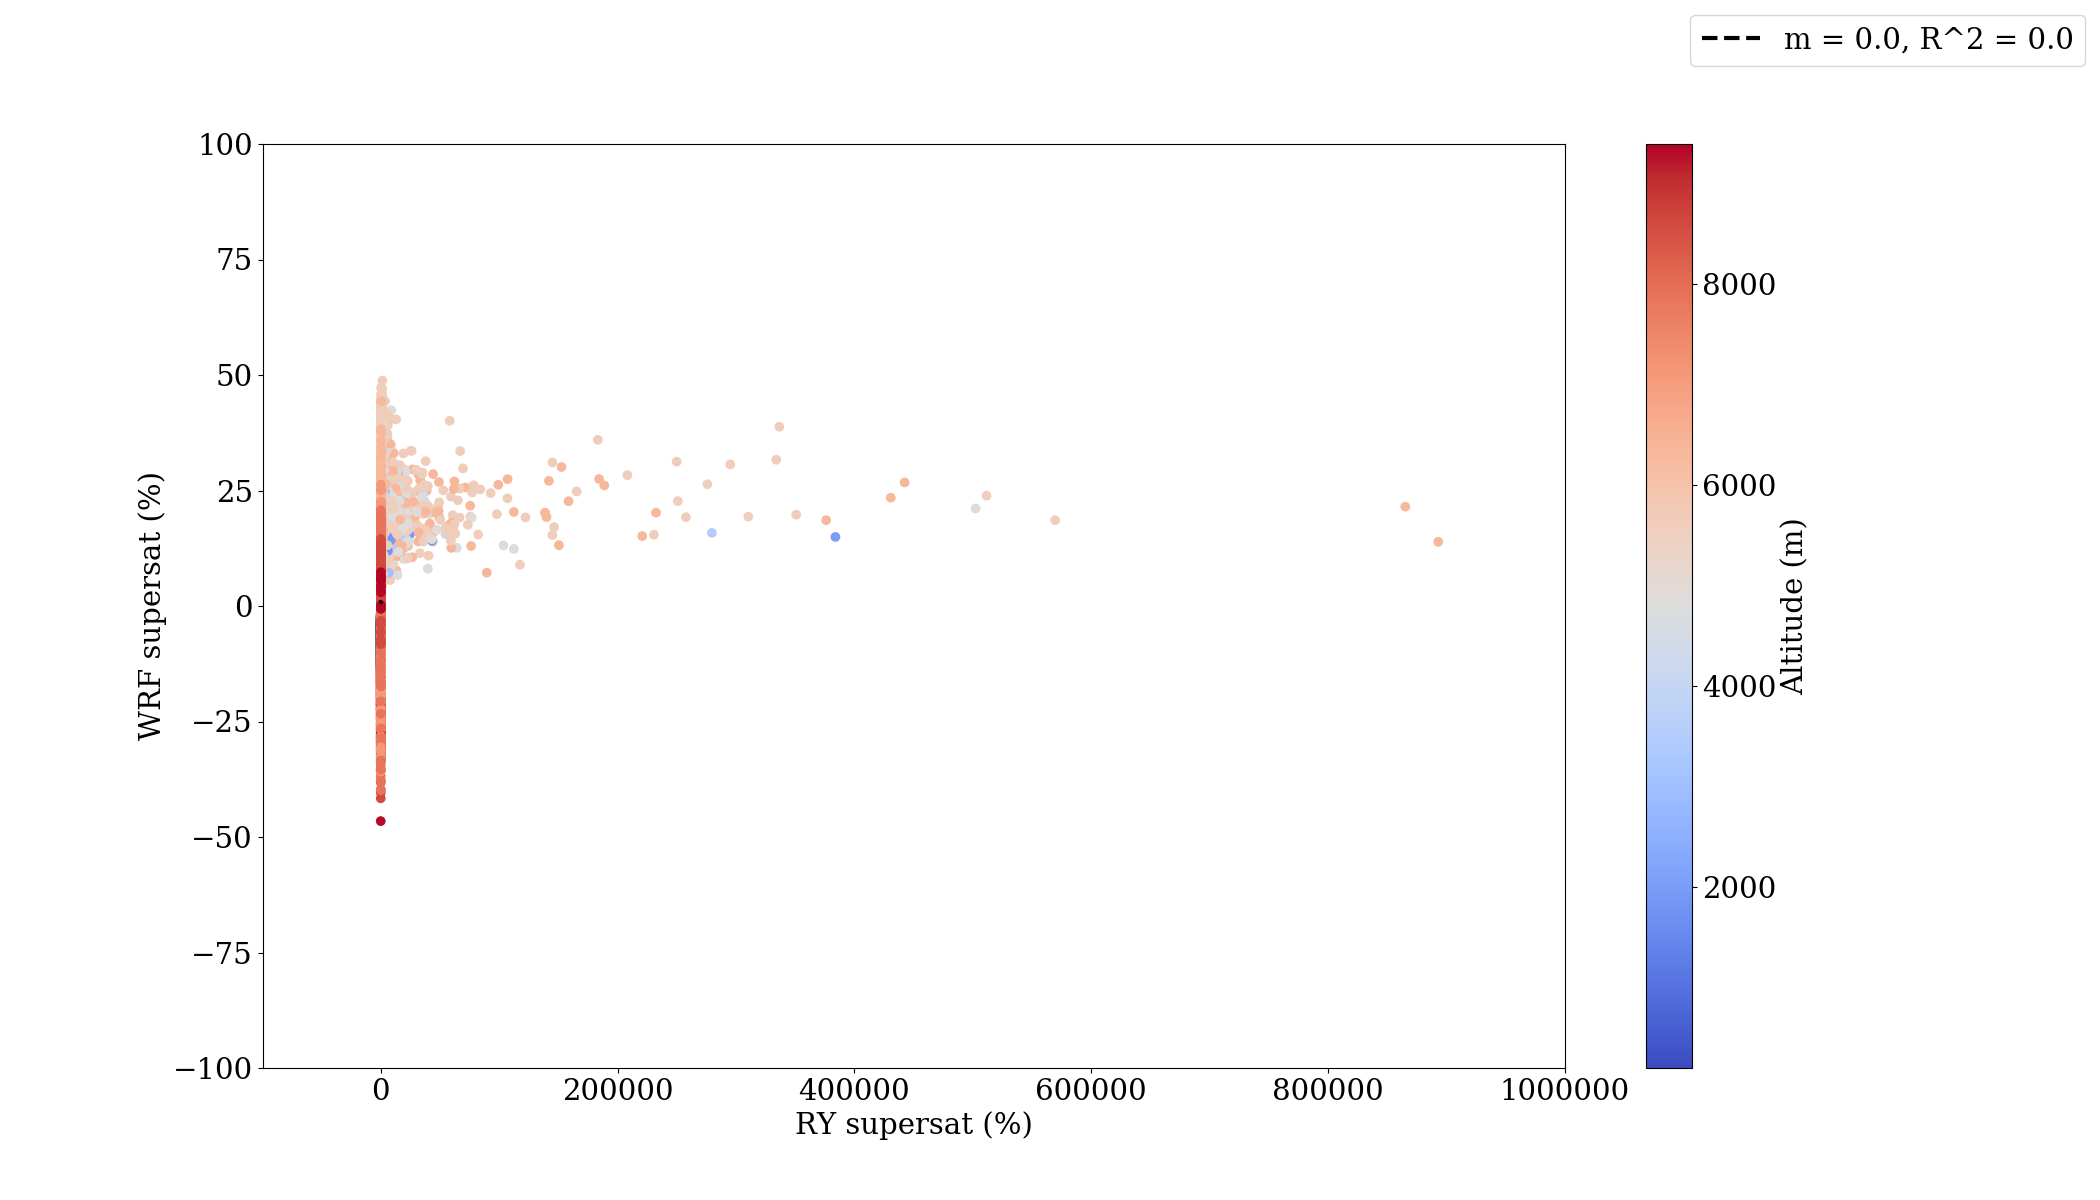
\includegraphics[width=10cm]{mywrf/v40_backtrack_qss_Unpolluted_figure.png}
    \caption{Same as Figure (\ref{v39unpol}), but with the full domain.}
    \label{v40unpol}
\end{figure}

\end{document}
